\chapter{Analysis}

Before going over the actual programming of the framework, we need to further inspect some of the features we have specified in the Introduction in Chapter \ref{Intro}. In this chapter, we will analyze features of this thesis, as well as suggest ways of solving problems, and in case there are more solutions, we will select the most suitable one with a proper explanation.

\section{Command System}
The most distinguishing feature of any game is its interactivity, and point-and-click adventure games are no different. We have already established the most common types of command systems in Chapter \ref{Intro} but now we need to design the command system according to our requirements \ref{intro:req:com_pan} - \ref{intro:req:mix}. 

One option is to split the controls into two separate systems, context-based and action-based, but that would make it difficult to mix them, which we need per requirement \ref{intro:req:mix}. Instead, we can build a single, unified framework that flexibly supports both modes.

Let us begin with the action-based command system, since its requirements are clear: we need a way to define actions and display their corresponding buttons in the UI. Once that core system is in place, we can incorporate situation-based controls. Notice that a situation-based system really offers only one action (let us call it \textit{Default}), which could simply be another entry in our action list. In other words, by treating \textit{Default} as just another action, our one command system can drive both explicit, multi-button interactions and context-sensitive, giving developers the freedom to mix and match however they like.

\subsection{Command structure}
\label{Analysis:CommandStructure}
As introduced in Section \ref{ActionPanel}, we want to display a sentence that clearly communicates what the character is about to do. To achieve this, we need a system that can dynamically build these sentences based on the player's input as well as react to the input appropriately.

Typically, there are three main sentence structures that emerge from combining command verbs with objects in the game world:
\begin{itemize}
    \item \verb|(verb)|, e.g. “\texttt{Walk to}”
    \item \verb|(verb noun)|, e.g. “\texttt{Look at poster}”
    \item \verb|(verb noun connector noun)|, e.g. “\texttt{Use key with lock}”
\end{itemize}

Each of these sentence structures requires a different number of inputs from the player. For example, the command “\texttt{Look at}” needs just a single object to complete the sentence, whereas “\texttt{Use}” requires two: an item and a target. Because of this, each command must define a rule that determines how many objects are needed and how they should be combined to form a meaningful interaction.

Generally, the verb always appears at the beginning of the sentence. What follows can either be nothing or a noun (i.e., a game object). The only common case where nothing follows the verb is with the command “\texttt{Walk to}.” This form is used when the player clicks somewhere in the scene that is not associated with any specific object, usually just to move closer to that point. Every other verb we have encountered is typically followed by at least one noun. Interestingly, “\texttt{Walk to}” can also be used in the \verb|(verb noun)| structure (e.g., “\texttt{Walk to poster}.”). Because of this flexibility, we can treat “\texttt{Walk to}” as a special case and consider it to be part of the \verb|(verb noun)| category for consistency.

From there, the sentence can either end or continue with a connector followed by another noun. The connector (e.g., “with”) links the two objects and indicates how they are meant to interact.

In general, when looking at sentence structures, we can work with nouns and connectors. While the connector is purely visual and tells us nothing about the logic of the command, the number of nouns is essential to detect when the game should react and execute an action when clicking on an object. 

\subsection{Logic system}
Each object in the scene needs to know how to react when a certain action is chosen. This means that when interacting with objects in the game, the player must follow a sequence of actions in order to progress, namely, meeting certain requirements. For example, only when having enough money can the player buy a map in the Secret of Monkey Island. This means that we need to create a logic system.

We need to define a list of actions that are triggered only under certain conditions, such as combining two items, giving an item to a character, or using an item to unlock something. These scenarios typically require interacting with at least one object beforehand. For instance, consider the example from Beneath a Steel Sky shown in Figure \ref{fig:Logic-BaSS}, where the player attempts to use a metal bar on a door. In this case, the metal bar is the previously selected object and the door is the one currently being interacted with.

\begin{figure}[H]
\centering
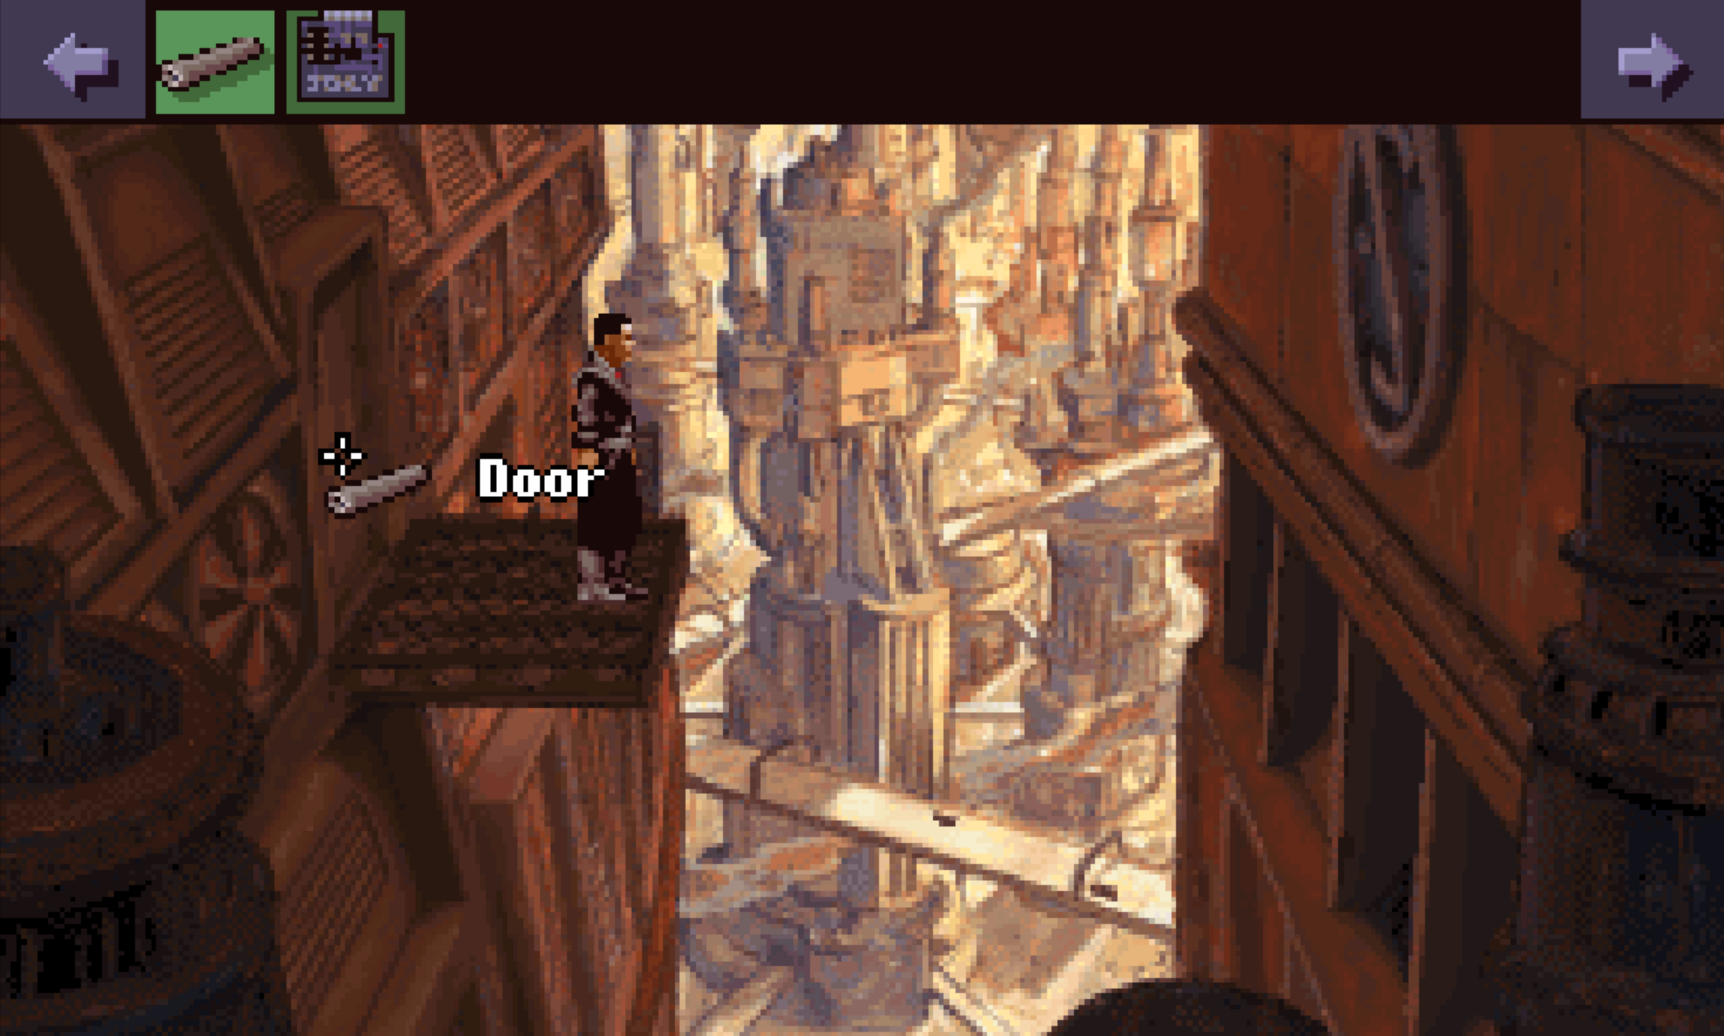
\includegraphics[width=.8\linewidth]{img/C-BaSS.png}
\caption{Beneath a Steel Sky: Using an object (a metal bar) on another object (a door).}
\label{fig:Logic-BaSS}
\end{figure}

When defining which items can be used on which objects, it is important to keep the logic organized, as this kind of system can become complex quickly. It makes the most sense to associate these interaction rules with the final object—the one currently being targeted. So, in the example above, the door object should contain the logic for what happens when the metal bar is used on it. Although it is technically possible to store this information on the metal bar instead, organizing it from the perspective of the final object is often more logical. It shifts the question from “What other items does this item interact with?” to “What items are needed to interact with this object?” We will refer to these first-selected items as \textit{Previous Interactables}.

Finally, some actions may depend on additional conditions, such as whether the player has enough money or has spoken to a certain character. In these cases, the player does not need to use an item. Instead, different actions can occur under various conditions. We will refer to these simply as \textit{Conditions}.

In the end, we obtain the system depicted in Figure \ref{fig:Logic:Diagram}. On the left, we have the \textit{Commands} that define the possible verbs such as “\texttt{Use}”, “\texttt{Talk to}”, “\texttt{Pull}” etc. Then there is an item which contains the possible \textit{Actions} assigned to each of the commands. Finally on the right we have two \textit{Actions}, each of them containing \textit{Previous Interactables}, \textit{Conditions} and the \textit{Actions} themselves. 

\begin{figure}[H]
\centering
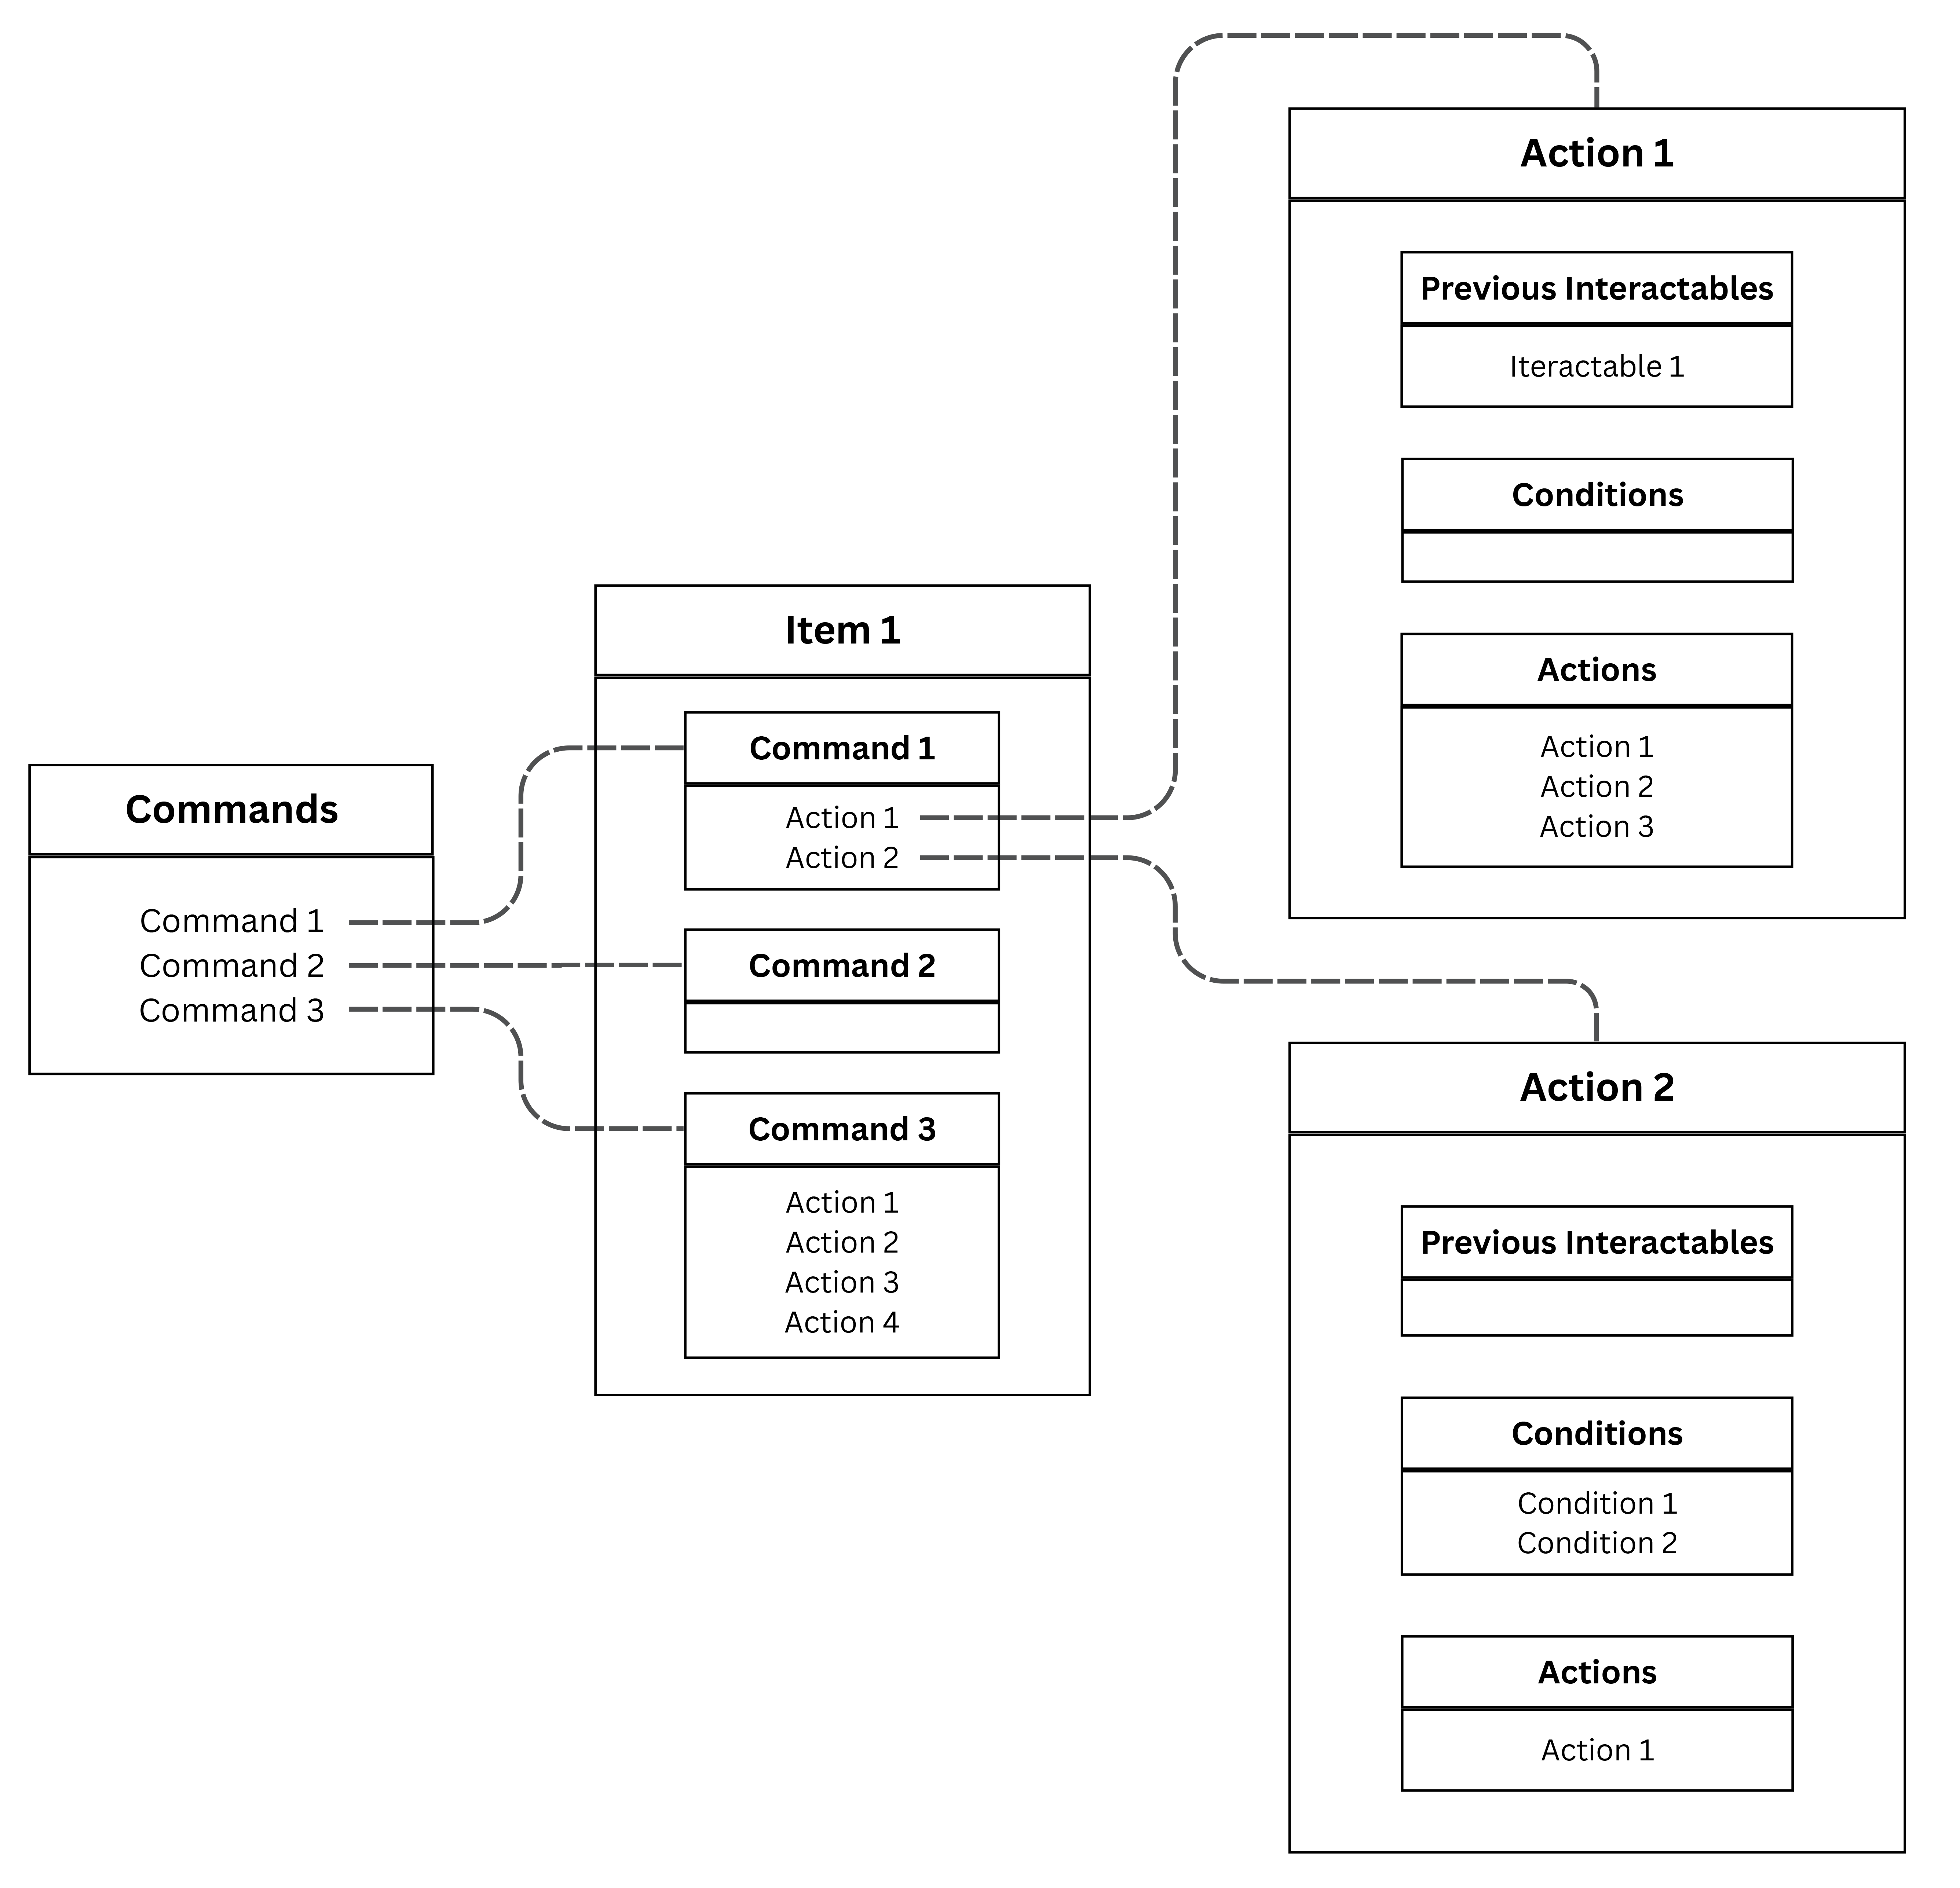
\includegraphics[width=0.8\linewidth]{img/Action-diagram.png}
\caption{Logic system.}
\label{fig:Logic:Diagram}
\end{figure}


\section{Walking system}
In Requirement \ref{intro:req:pathfinding}  we have established that the player should have the ability to move around the walking area. The development of the walking system could be divided into two main parts:
\begin{enumerate}
    \item The representation of the walkable area,
    \item The problem of finding the path to a goal.
\end{enumerate} 

\subsection{Walkable Area}
\label{analysis:walkableMap}

The characters in a video game exist in a defined in-game world. Naturally, this world needs boundaries and areas where the player can move and interact. The walkable area refers to the regions of the game world that the player is allowed to access and navigate. It often consists of a collection of rooms, but it could be just as easily a city square, a forest, or any other kind of space that the developer envisions. While it is easy to imagine these spaces and the areas accessible to the player in our minds, we need a clear and practical way to define them in the game engine. 

\subsubsection{Bitmap}
In his article, Steven Henk Don \cite{Shdon} outlines an approach to representing walkable areas using a walkability bitmap. This method involves creating an image composed of a limited set of colors, where each color conveys specific information about the game environment. In our case, this bitmap would describe the possible walkable areas that the player may traverse. Figure \ref{fig:WS:Bitmap} shows one such bitmap on top of the scene. In this example, the player is able to freely walk around the area highlighted with green color, while the dark areas are inaccessible. Finally, the player can step on the blue area only when certain conditions are met (e.g. after talking to the bouncer).  

\begin{figure}[H]
\centering
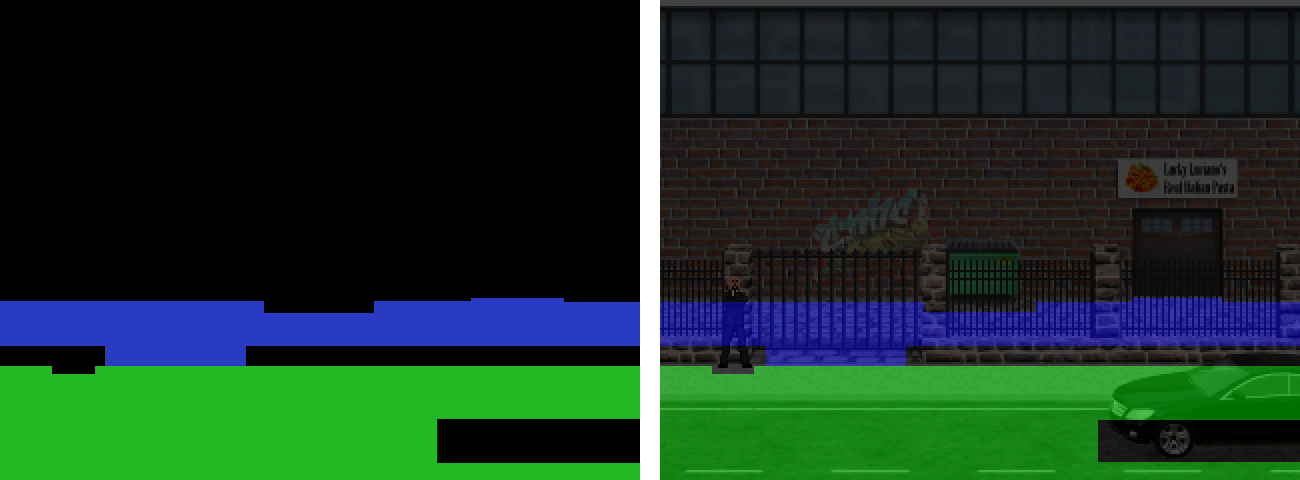
\includegraphics[width=1.0\linewidth]{img/walkability-map2.png}
\caption{Walkability bitmap: bitmap mask (left) and mask applied on top of a scene (right). Source \cite{Shdon}.}
\label{fig:WS:Bitmap}
\end{figure}

To obtain such a bitmap, the user must use image-editing software to manually create colorful shapes that represent the accessible parts of the environment and then save the image. Additionally, modifying the bitmap is difficult and time-consuming, as it requires reopening the editing software and making manual changes. Our goal is to find a solution that can be integrated directly into the framework while keeping the experience user-friendly, something this approach does not support. 

\subsubsection{Sierra's approach}
Since Chapter \ref{Intro} focused heavily on the features of classic point-and-click games, it makes sense to now examine how walking systems are implemented by prominent studios. Unfortunately, there is limited publicly available information on this topic, possibly due to the existence of patents or proprietary techniques that are not openly shared. However, we have found one notable example. According to ScummVM, an open-source project that reimplements classic game engines, a prominent game company Sierra behind classics such as \textit{King's Quest} implemented their own patented pathfinding algorithm designed to navigate game characters around obstacles \cite{ScummVM-polygons}. It uses polygons to represent the area as well as obstacles, which can be divided into four types with the following rules:
\begin{itemize}
    \item  \textit{Barred access polygons} strictly block entry, meaning if the end point lies inside one, the path ends at the nearest point on the polygon’s boundary. 
    \item On the other hand, \textit{total access polygons} are ignored if the start or end point is inside them, allowing paths to begin or end there, but otherwise preventing entry. \textit{
    \item Near-point access polygons} require that the path enters or exits through the closest boundary point (near-point) if the start or end lies inside. 
    \item Finally, \textit{contained access polygons} define strict boundaries inside which the entire path must remain. It means that if the end point lies outside, the path stops at the near-point. Since polygons cannot intersect, only one contained access polygon can exist in a scene.
\end{itemize}

While this method is more useful and usable in the Unity engine, it also introduces additional polygon types to support more nuanced navigation behavior. However, these specialized polygons appear to add unnecessary complexity, as the same results, such as adjusting start or end points to valid locations, can be achieved through simpler methods. Unity supports storing data in game objects and these additional rules can be simply integrated this way. Therefore, this thesis will adopt some ideas from Sierra’s method, but will not implement multiple polygon types, in favor of a more user-friendly solution. So let us examine one more approach, which will make us understand the method used in our framework.

\subsubsection{Polygons}
\label{Analysis:Polygon}
A way to represent the walkable area is discussed in detail in articles by Mic Uurloon \cite{Uurloon1}\cite{Uurloon2}, where walkable areas and obstacles are defined using polygon shapes directly in the Unity engine. The idea is to have one primary shape that defines the main walkable area, be it a room, a hall, or a town square. Inside that area, there can be places that are not accessible currently or indefinitely (e.g. furniture), let us call them obstacles. We can define the boundaries of the walkable area and the obstacles using polygons, as seen in Figure \ref{fig:WS:Poly}. One such polygon can be used to outline the primary area where the user walks around, while additional polygons can be viewed as obstacles that the player must avoid.

\begin{figure}[H]
\centering
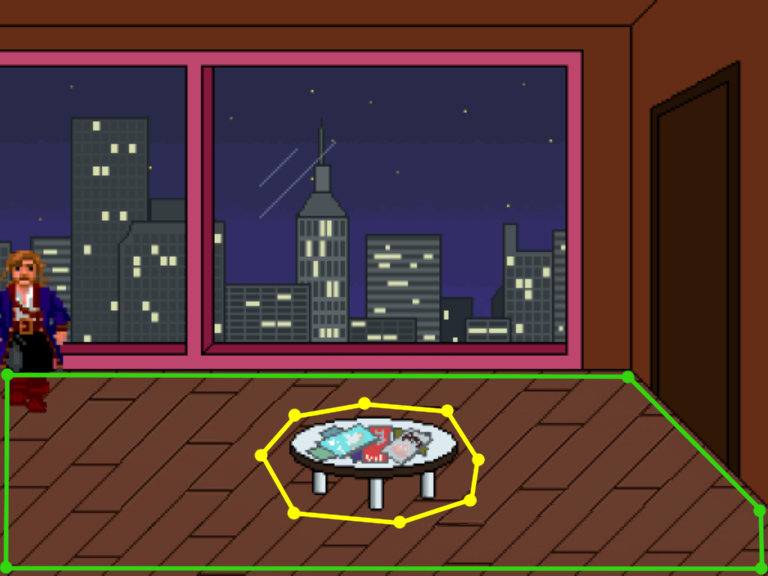
\includegraphics[width=.7\linewidth]{img/WS-polygons4.png}
\caption{Polygonal map: the room as the main walkable area (green) and the table as an obstacle (yellow). Source \cite{Uurloon1}.}
\label{fig:WS:Poly}
\end{figure}

The main advantage of this approach is the ability of the user of the framework to modify the shapes on the fly whenever necessary. Next, this system can be implemented directly in Unity and does not require any other software to set it up. Given these benefits, this will be the primary approach explored and implemented in this thesis. 


\subsection{Pathfinding}
A crucial part of character movement is the ability to find a path to the goal.

\subsubsection{NavMesh}
Developers familiar with Unity’s pathfinding tools may know about NavMesh, a system that generates a mesh to represent walkable surfaces and obstacles in a 3D environment, while also supporting AI navigation. While powerful in 3D projects, NavMesh presents challenges in 2D development, as Unity's 2D space uses the X and Y axes, whereas NavMesh operates on the XZ plane. Some open-source projects, such as NavMeshPlus, extend the NavMesh functionality to 2D environments. However, NavMeshPlus is a complex and feature-rich project, which can be overwhelming for beginners and includes functionality beyond the needs of simpler projects. For this reason, a more lightweight and user-friendly alternative should be considered, which prioritizes ease of integration and clarity over extensive feature sets. So let us look at this problem from the beginning.

\subsubsection{Straight line}
The simplest option is to take a direct line to the goal. However, this approach drastically restricts the types of walkable areas. Firstly, the walkable area is restricted only to convex shapes, where any two points can be connected by a straight line that is entirely contained inside that shape. However, if the walkable area is concave, some vertices point inward, creating obstructions that block direct visibility between points, as depicted in Figure \ref{fig:Polygons}. In the convex polygon on the left, any two points can be connected by a straight line that remains entirely inside the boundaries of the shape. In contrast, the polygon on the right is not convex, and as a result the line connecting points B and D exits the shape. 

\begin{figure}[H]
\centering
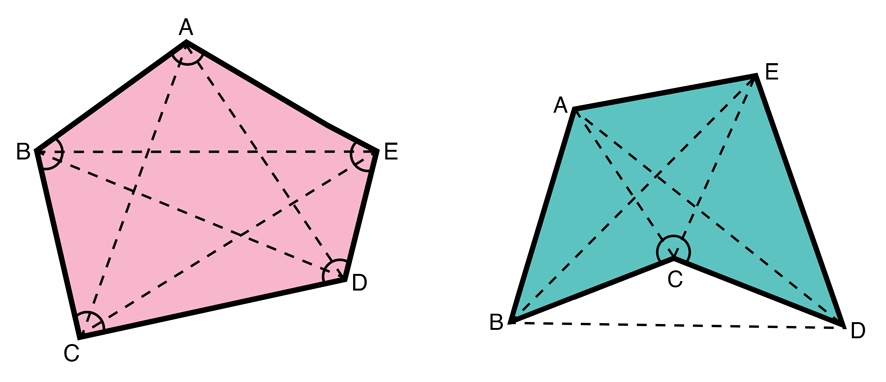
\includegraphics[width=.8\linewidth]{img/polygons.png}
\caption{Convex (left) and concave (right) polygons. Source \cite{Polygons}.}
\label{fig:Polygons}
\end{figure}

But it is not just the shape of the main walkable area that poses limitations. The idea of placing obstacles inside that area introduces a challenge, as a straight line alone cannot accurately represent the action of navigating around such objects. This means that areas like the ones in Figures \ref{fig:Path-B}  and \ref{fig:Path-M}  cannot be replicated. In both of the Figures, a character is tasked to move along the straight blue line. However, either the polygon of the walkable area itself (Figure \ref{fig:Path-B}) or another polygon (Figure \ref{fig:Path-B}) pose as a block, shown by the dotted line segment.

\begin{figure}[H]
\centering
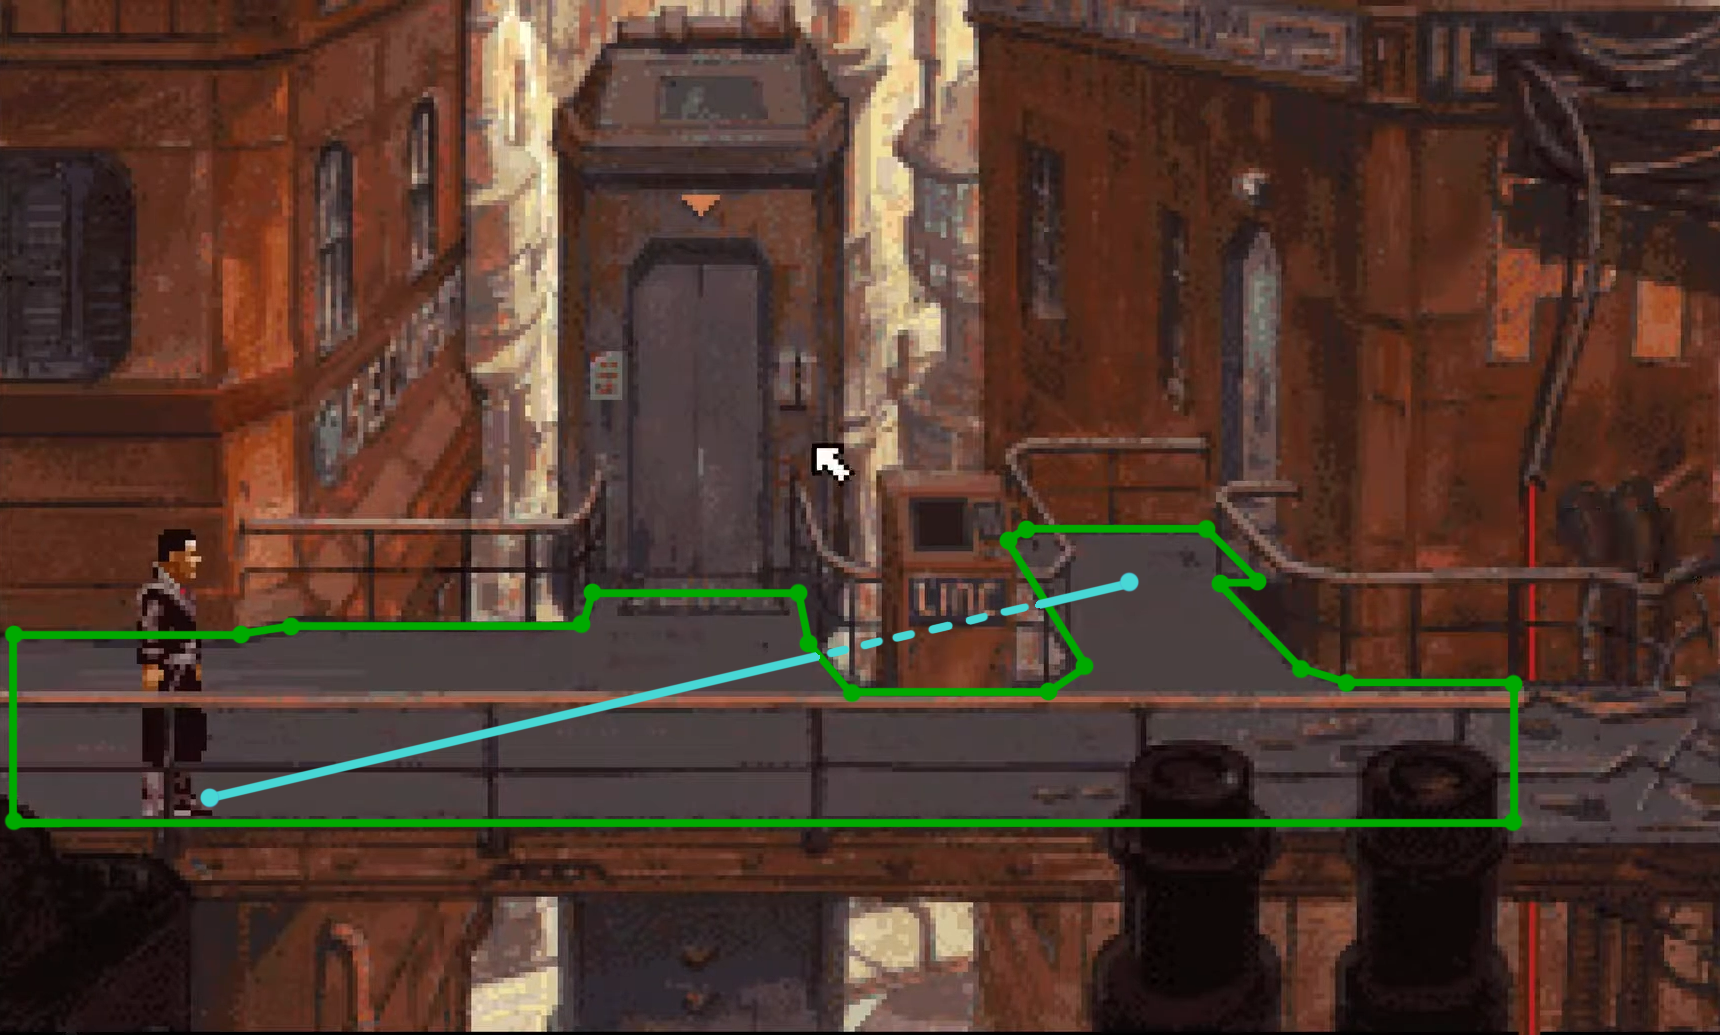
\includegraphics[width=.7\linewidth]{img/Path-BaSS2.png}
\caption{Beneath a Steel Sky: A concave path where no one straight line would access each point from where the character is standing.}
\label{fig:Path-B}
\end{figure}

\begin{figure}[H]
\centering
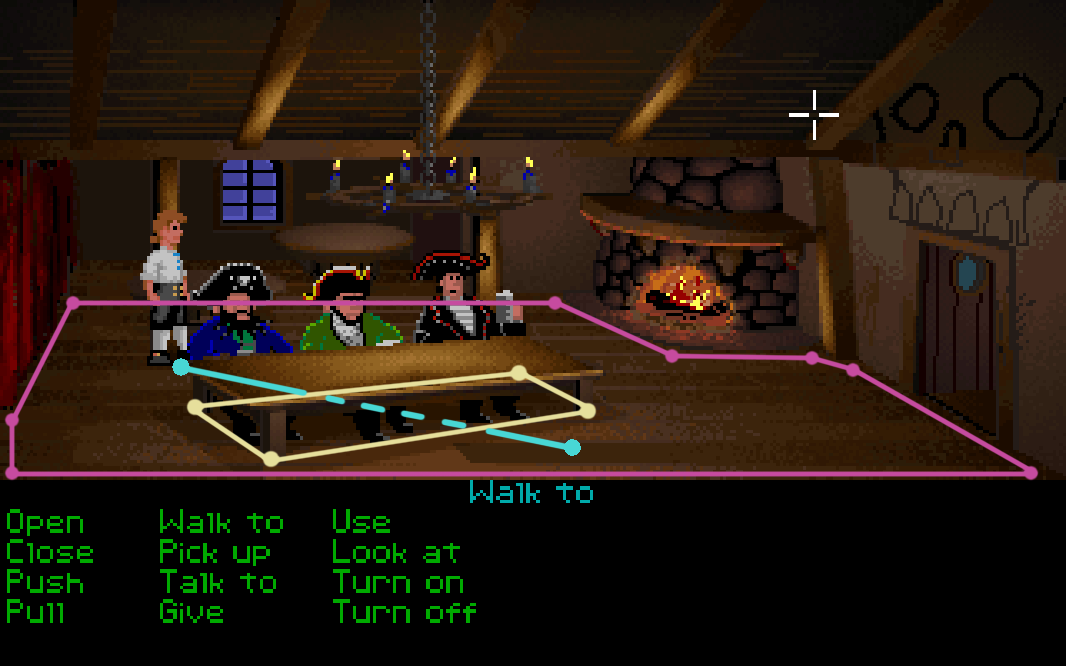
\includegraphics[width=.7\linewidth]{img/Path-TSoMI2.png}
\caption{The Secret of Monkey Island: An obstacle (table) in the middle of the room restricts the player's access to the other part of the room.}
\label{fig:Path-M}
\end{figure}

\subsubsection{Multiple line segments}
So if one straight line is not enough, we can break it into smaller line segments. This way of dividing the path into smaller sub-paths allows the character to get to the goal while being restricted to the walkable area. But now the question is which lines we should choose.

We might intuitively imagine an algorithm that first attempts to follow a straight line toward the goal. When an obstacle approaches, whether it is the edge of the walkable area or an internal obstacle, it would try to move sideways and find a way around it. While this seems like a reasonable approach, it does not truly solve the core problem: finding an actual route. Instead, it merely postpones the decision-making. So what are our options?

A naive strategy would be to follow the edge of the obstacle, either to the left or to the right, until a straight line to the goal becomes possible again. If another obstacle is encountered, the process is repeated. However, this approach glosses over a critical point: How do we decide which direction to follow? Picking a random direction can lead to highly inefficient paths. Figure \ref{fig:Path-P} highlights a situation in which the goal is to get from point A to point B. However, the direct path (blue) is obstructed by an edge of the polygon itself. Looking at the figure, we can see that the following red path causes an unnecessary detour, making the movement appear unnatural. Ideally, we want the path to look natural and intuitive, similar to the green path.

\begin{figure}[H]
\centering
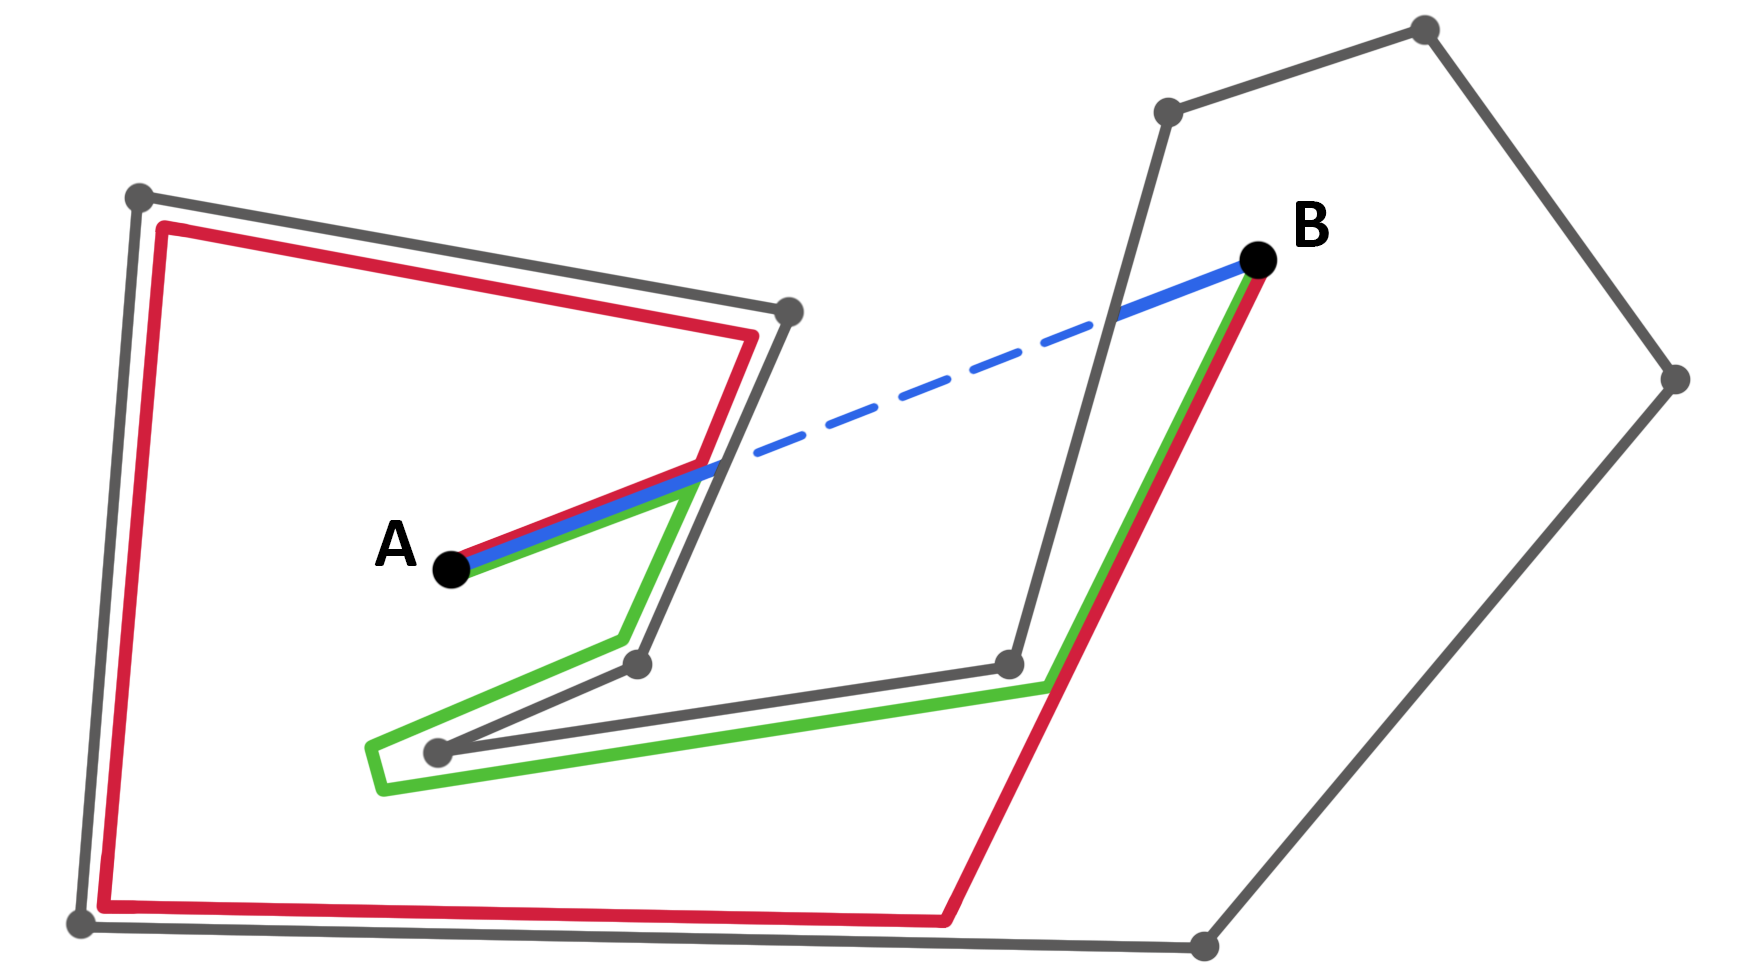
\includegraphics[width=.65\linewidth]{img/polygon-prototyp.png}
\caption{Pathfinding in a concave polygon - simple approach}
\label{fig:Path-P}
\end{figure}

\subsubsection{Shortest path}
In real life, people instinctively aim for the shortest or most efficient route. By comparing the left and right paths in Figure \ref{fig:Path-P}, we can identify the shorter one - likely the more natural and visually appealing choice. But even this can be improved. If we examine the start of the path, our algorithm initially attempts to move straight toward the goal until hitting an obstacle. However, a person would probably try to avoid the obstacle from the beginning and aim to take the shortest path right away. That is the key point: instead of reacting to obstacles as they come, we should aim to find the shortest path from the start, just like the one in Figure \ref{fig:Path-P2}.
 
\begin{figure}[H]
\centering
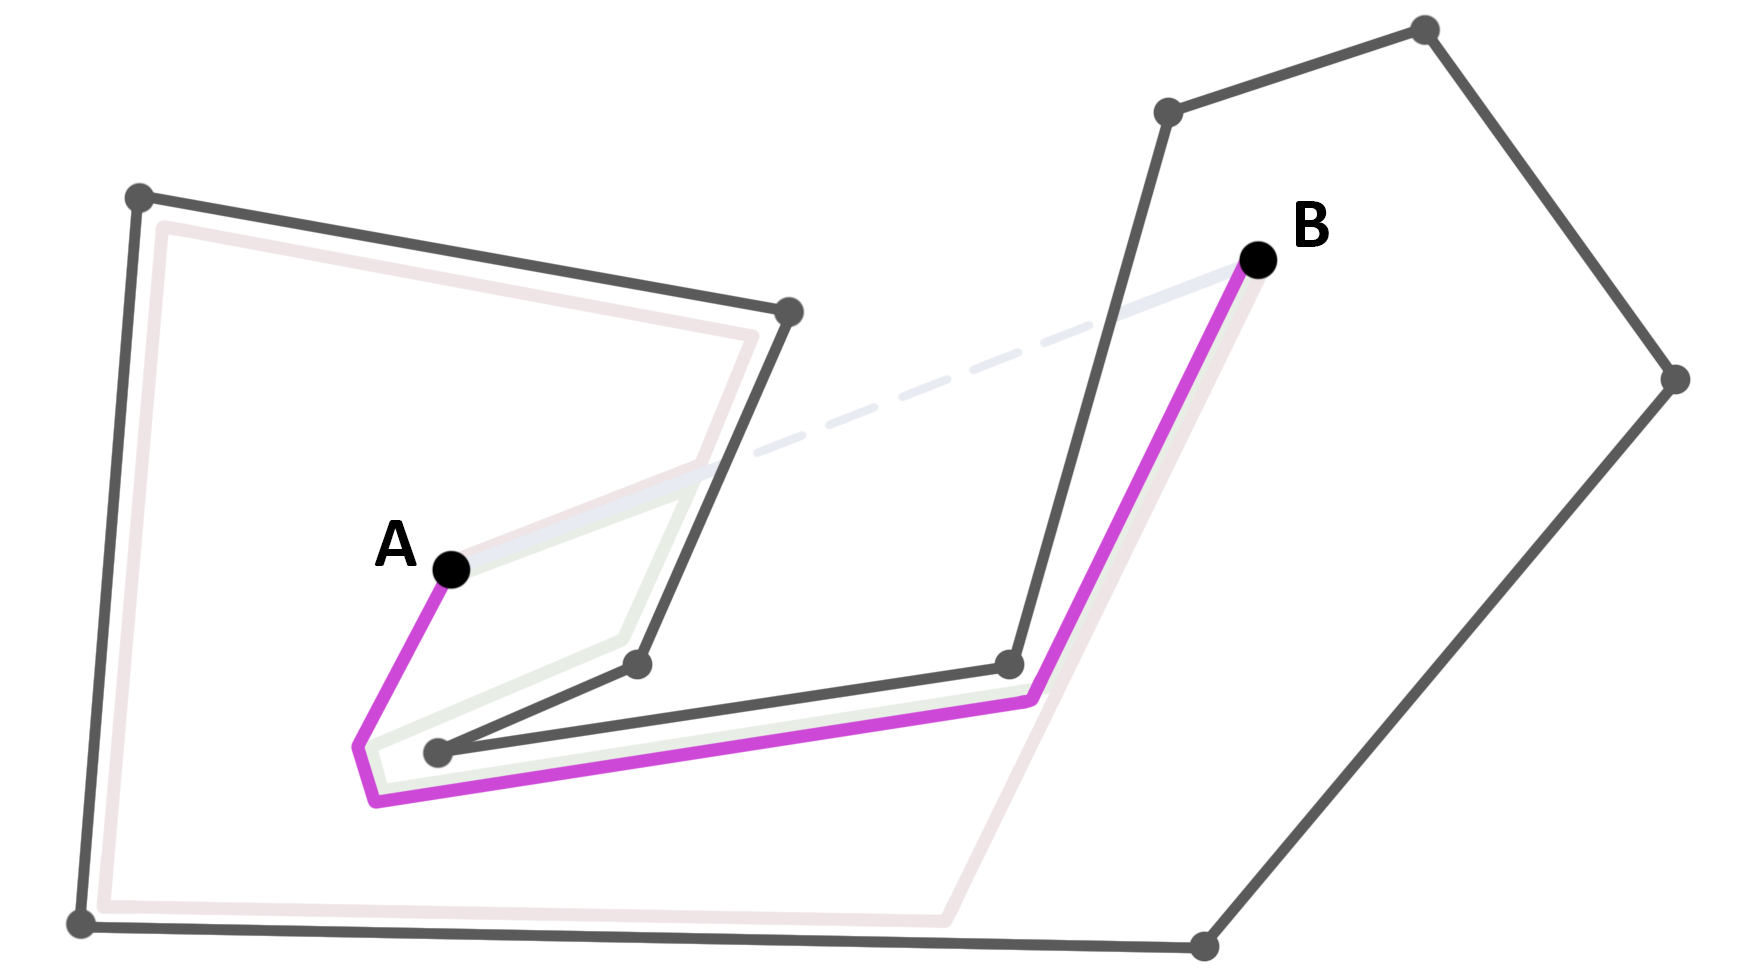
\includegraphics[width=.65\linewidth]{img/polygon-prototyp2.png}
\caption{Pathfinding in a concave polygon - shortest path}
\label{fig:Path-P2}
\end{figure}

When it comes to choosing a pathfinding algorithm, our goal is to find one that reliably and efficiently determines the shortest path between two points in a 2D space. Since our maps typically contain only a few dozen vertices, raw performance is not a critical concern. Among the most commonly used algorithms in game development is A*, known for its balance of simplicity and efficiency. While our thesis does not demand high performance, A* still meets all our needs and is straightforward to implement. Moreover, if the project were to scale and require handling more complex maps with a larger number of vertices, A* would still be a solid choice due to its proven performance. 

A key component of the A* algorithm is the heuristic function which estimates the cost of the cheapest path to the goal. If the function never overestimates it, A* is guaranteed to return one of the shortest paths from start to goal. For the purpose of free character movement on a 2D plane, the Euclidean distance was chosen as a heuristic function. It is well suited for point-and-click adventure games, where characters can move freely in any direction, making straight-line distance a natural and accurate estimate of travel cost.  It can be calculated from the Cartesian coordinates of the points while also applying the Pythagorean theorem:

\[
d = \sqrt{(x_2 - x_1)^2 + (y_2 - y_1)^2}
\]

%\subsubsection{Sierra}
%A very similar approach was also used in Sierra's engine with multiple levels of optimization that essentially aim to find the shortest path to the goal \cite{ScummVM-patent}. The algorithm consists of three distinct phases: pre-processing, pathfinding, and post-processing. In pre-processing, the input is adjusted so that start and end points are not inside any polygons, with special rules for total and near-point access polygons. Post-processing then reattaches any final segments. The pathfinding phase begins by attempting a straight-line path from start to end and rerouting around any intersected polygons. At optimization level 0, the algorithm simply detours along the shortest boundary path between the first and last intersection points of a polygon. Optimization level 1 improves this by attempting shortcuts between path nodes, as long as they do not intersect any polygons. Level 2 further enhances this by testing all possible combinations of routes around each polygon to find the shortest overall path. However, this exhaustive approach still does not guarantee a globally shortest path in all cases, as it only considers polygons intersected by the initial straight trajectory. Because of this, we will rather use the previous method as it provides us with a stable solution and a guarantee of the shortest path.


%Objects typically get there by taking the shortest route possible. This makes sense in point-and-click adventure games, as player input is intentional and direct: clicking on a location implies that the character should move there efficiently, without unnecessary detours. The problem of finding the shortest path is a well-studied field in computer science, with several established algorithms designed to solve it. 

\subsubsection{Weighted Graph}
\label{Analysis:Graph}
Polygons only serve as a visual representation of the walkable area to the framework users. However, in order for the algorithms to work, the walkable area must also be represented in a suitable form for computation. Specifically, if we want to determine the shortest path to a destination, we need a way to calculate the distances between the points. Without this, identifying the optimal route would be impossible. A weighted graph provides an ideal structure for this purpose. It consists of nodes connected by edges, each assigned a non-negative value representing the distance between them. That said, generating a graph that includes every possible node and edge would be both inefficient and impractical. The approach for creating a graph from polygons that was used in our thesis was adapted from the articles by Mic Uurloon. Details about this method together with more interactive examples explaining how the algorithm works can be found in his articles Part 1 \cite{Uurloon1} and Part 2 \cite{Uurloon2}, which further reference an article by David Gouveia \cite{Gouveia}.
Figure \ref{fig:Graph}
showcases a graph created using Uurloon's method.
\begin{figure}[H]
\centering
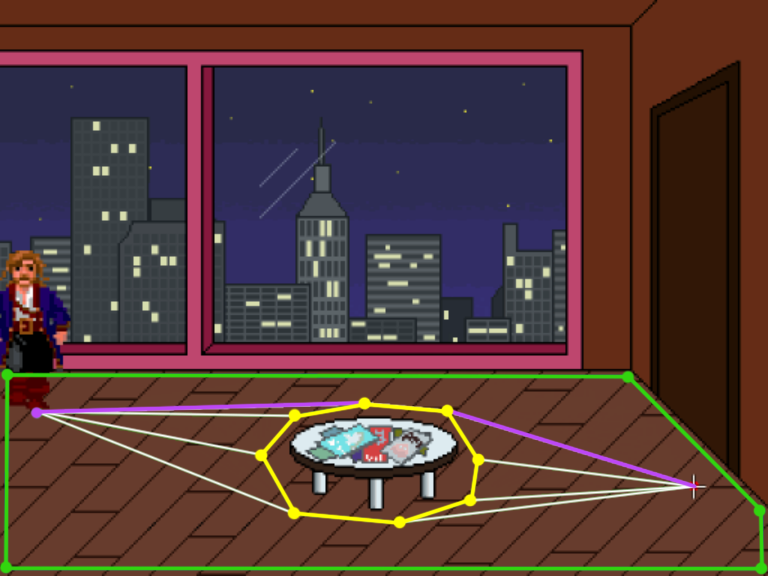
\includegraphics[width=.7\linewidth]{img/WS-polygons3.png}
\caption{Graph: Walkable area consisting of polygons (green and yellow) and a graph (white) with a possible path (violet). Source \cite{Uurloon1}.}
\label{fig:Graph}
\end{figure}


\section{Depth Simulation}
As we have specified in Requirements \ref{intro:req:scale} and \ref{intro:req:layers}, we want to simulate the feeling of a 3D space. 

\subsection{Scaling}
\label{analysis:depth:scaling}
The human eye perceives depth by observing objects in the distance as smaller than they actually are. There are a number of ways we can simulate this phenomenon in a 2D video game. The following three approaches are listed in Mic Uurloon's article about scaling actors \cite{Uurloon3}. We will look closely at them and choose a suitable option for our framework.

\subsubsection{Axis-based scaling}
One option would be to scale the size of the character based only on the Y coordinates. This way, we can set the boundaries for the minimum and maximum scale of the moving object in the given area, and then, based on the distance from those boundaries, set the appropriate value, visualized in Figure \ref{fig:Room} . 

\begin{figure}[H]
\centering
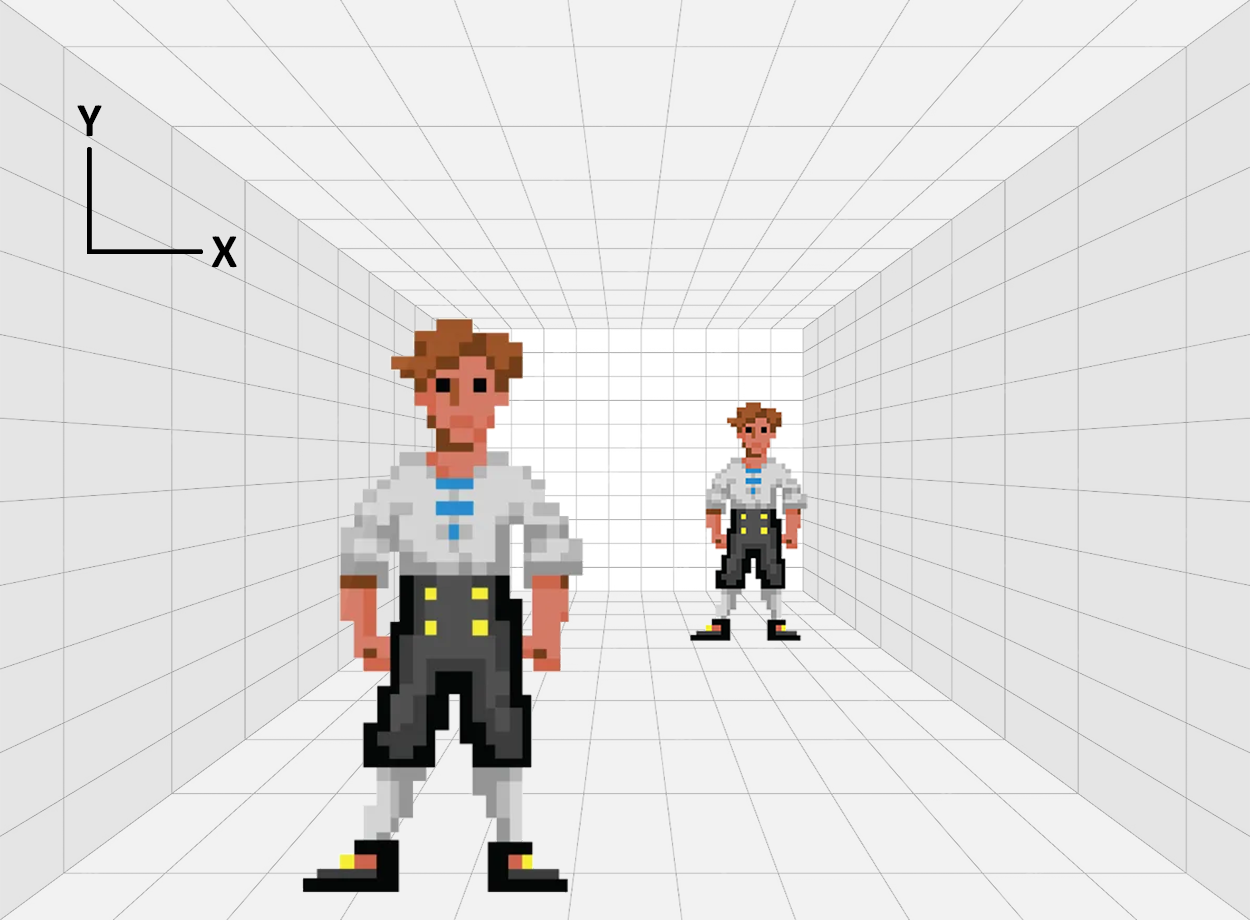
\includegraphics[width=.55\linewidth]{img/room2.png}
\caption{Character scaling by Y axis—success.}
\label{fig:Room}
\end{figure}

This approach is very simple, which is both its advantage and its disadvantage. Although it is easy to implement, it is not possible to achieve more complex scenes in which a character's sprite scales dynamically independently of the Y coordinates, such as the example in Figure \ref{fig:ScaleF}. Although both characters share the same Y-coordinate, the overall image appears off. Due to the perspective of the corridor on the right side of the figure, one character looks disproportionately large and unnatural.  A similar problem would arise with only considering the X coordinates.

\begin{figure}[H]
\centering
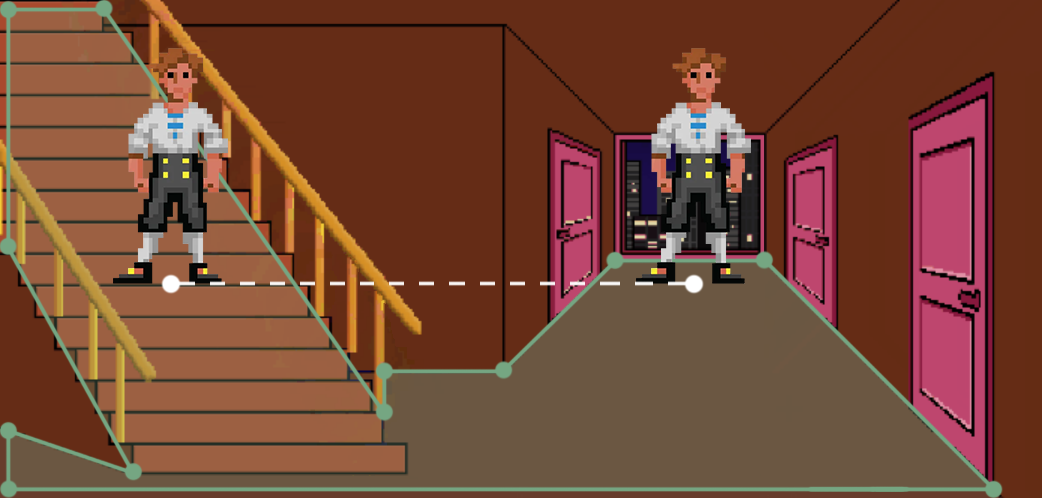
\includegraphics[width=.75\linewidth]{img/scalef-y.png}
\caption{Character scaling by Y axis—fail. Source \cite{Uurloon3}}
\label{fig:ScaleF}
\end{figure}

\subsubsection{Vertex-based scaling}
Our goal is to dynamically scale the character sprite based on its position on the map. To achieve this, we need a system that adjusts the sprite’s size depending on its location. A suitable way to store this scaling data is by assigning it to the vertices of the polygons that define the walkable area. Each vertex could carry a floating-point value representing the desired scale at that point, allowing us to interpolate the character's size as it moves across the map.  An advantage is the fact that the developer could have a free range on the exact details of the area. However, modifying the scales is not that easy because one must go through the necessary nodes and change the factor essentially by hand. This approach is a bit more complicated than the previous ones, but still fairly simple to implement and doable entirely in Unity.

\subsubsection{Bitmap-based scaling}
Finally, it is possible to use a bitmap and map the alpha value of each pixel to a scaling factor (see Mic Uurloon's article \cite{Uurloon3} for more information). This would be very precise, as the developer can set it up exactly as they wish. However, we again come across the problem we discussed in Section \ref{analysis:walkableMap} where we made it clear that we prefer to implement features that can be simply modified inside Unity.

\subsubsection{Conclusion}
From these three approaches only two seem to be doable entirely inside the framework: Y scaling (optionally X scaling) and custom vertices scaling. We aim to implement both of them in the hopes of offering a wide variety of options to developers.

\subsection{Layering}
Next, let us examine the layering. Our aim is to dynamically adjust the visibility of objects, as seen in Figure \ref{fig:Layers}. The human eye and brain can process this kind of information in the real world naturally and can therefore create a visual image of how objects are ordered one after the other. Because we are working with a 2D space, we have to do a bit more work simulating this phenomenon and determining in what order the sprites of objects should be displayed. Fortunately, it is very simple since all we need is to look at the Y coordinates. If object A has a smaller Y coordinate than object B, it means that A should be drawn on top of B. This is not complicated, but also not trivial, since it would be necessary to perform this check between each two objects in the scene. Lucky for us, Unity offers tools for 2D renderer sorting \cite{Unity-sorting} and can therefore take care of this problem for us. What we are looking for is the Custom Axis sort mode \cite{Unity-customAxis} in Graphics section under the Project Settings window. Details on the setup with a couple more modifications to make it just right can be found online in the Sunny Valley Studio article \cite{Piotr} . 

\begin{figure}[H]
\centering
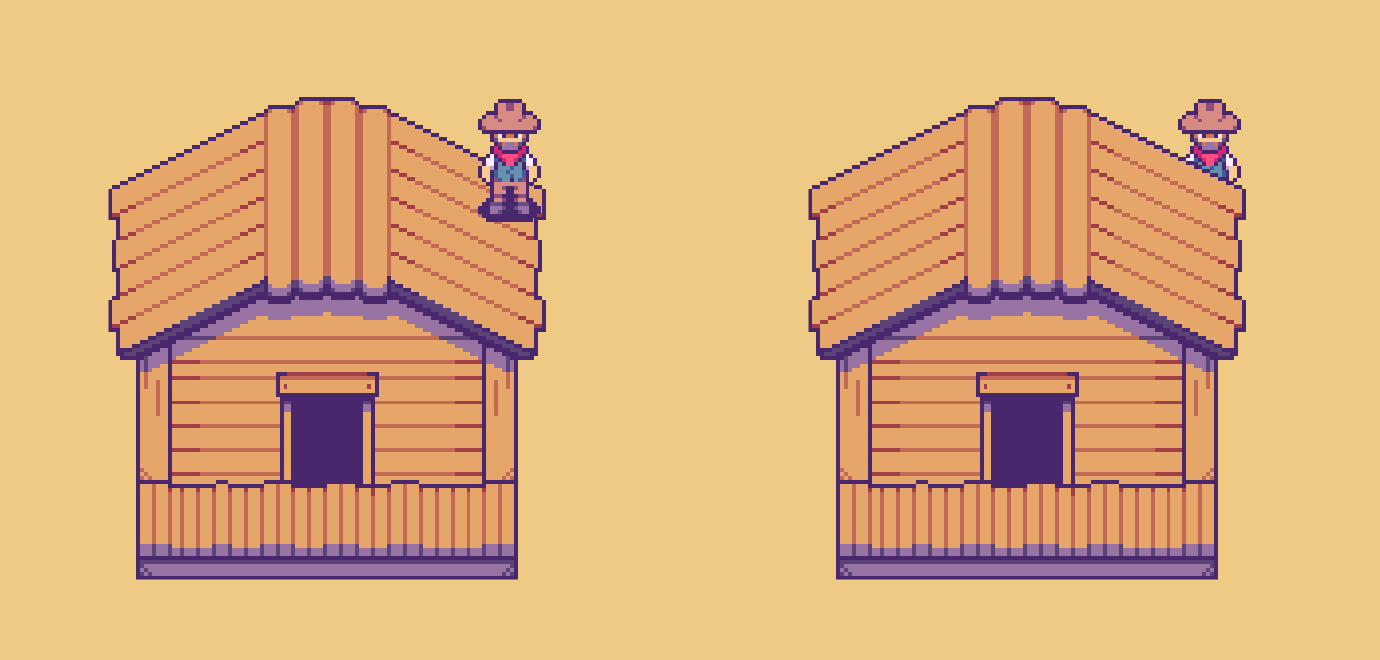
\includegraphics[width=.8\linewidth]{img/layers.png}
\caption{Wrong (left) and correct (right) 2D layer ordering. Source \cite{Piotr}.}
\label{fig:Layers}
\end{figure}

\section{Inventory System}
Collecting items and using them in the environment is a classic feature of point-and-click adventure games. To support this gameplay element, we need a system that makes it easy to define, collect, and use items. In order to meet the system's needs as well as the requirements listed in \ref{intro:req:inv_formats} – \ref{intro:req:tag}, each item no matter if it is located in inventory (\textit{inventory item}) or in the in-game world (\textit{world item}) should include the following data: \textbf{name}, \textbf{sprite} (image), \textbf{description}.
%\begin{itemize}
%\item a name,
%\item a sprite (image),
%\item a description.
%\end{itemize}

The name is used when the inventory is set to display item names, and can also appear as a tag when hovering over interactive items in the game world. The sprite is used when the inventory shows icons instead of names, in which case the visual representation alone is shown. Lastly, the description comes into play when the game needs to explain the item's function or purpose, as discussed further in Section \ref{sec:Inventory}.

An important aspect is the ability to reference these objects across different scenes. A very user-friendly approach is to implement them in Unity as \verb|ScriptableObject|s. This allows new items to be created easily inside the project and referenced globally across scenes.

There are countless ways to represent an inventory in the user interface. For instance, in Beneath a Steel Sky, the inventory appears by hovering the mouse at the top of the screen, after which it slides down into view. Because these kinds of interaction are often unique to a particular game, they will only be implemented in the prototypes and not as part of the framework itself. The framework will, however, include a general grid-based inventory structure, leaving specific stylistic or behavioral modifications to the developer.

\section{Dialogue System}
Conversations between characters help players understand the story and connect with the game world. While they usually take the form of a dialogue between two characters, that is not always the case. When only one character is speaking, it becomes a monologue or thinking aloud. On the other hand, conversations can also involve more than two characters, resulting in group interactions. 

There are cases where dialogue is limited to a simple exchange of lines without requiring player input, such as the first dialogue between Foster and Joey in Beneath a Steel Sky in Figure \ref{fig:DialogueSimple}. 

\begin{figure}[H]
\centering
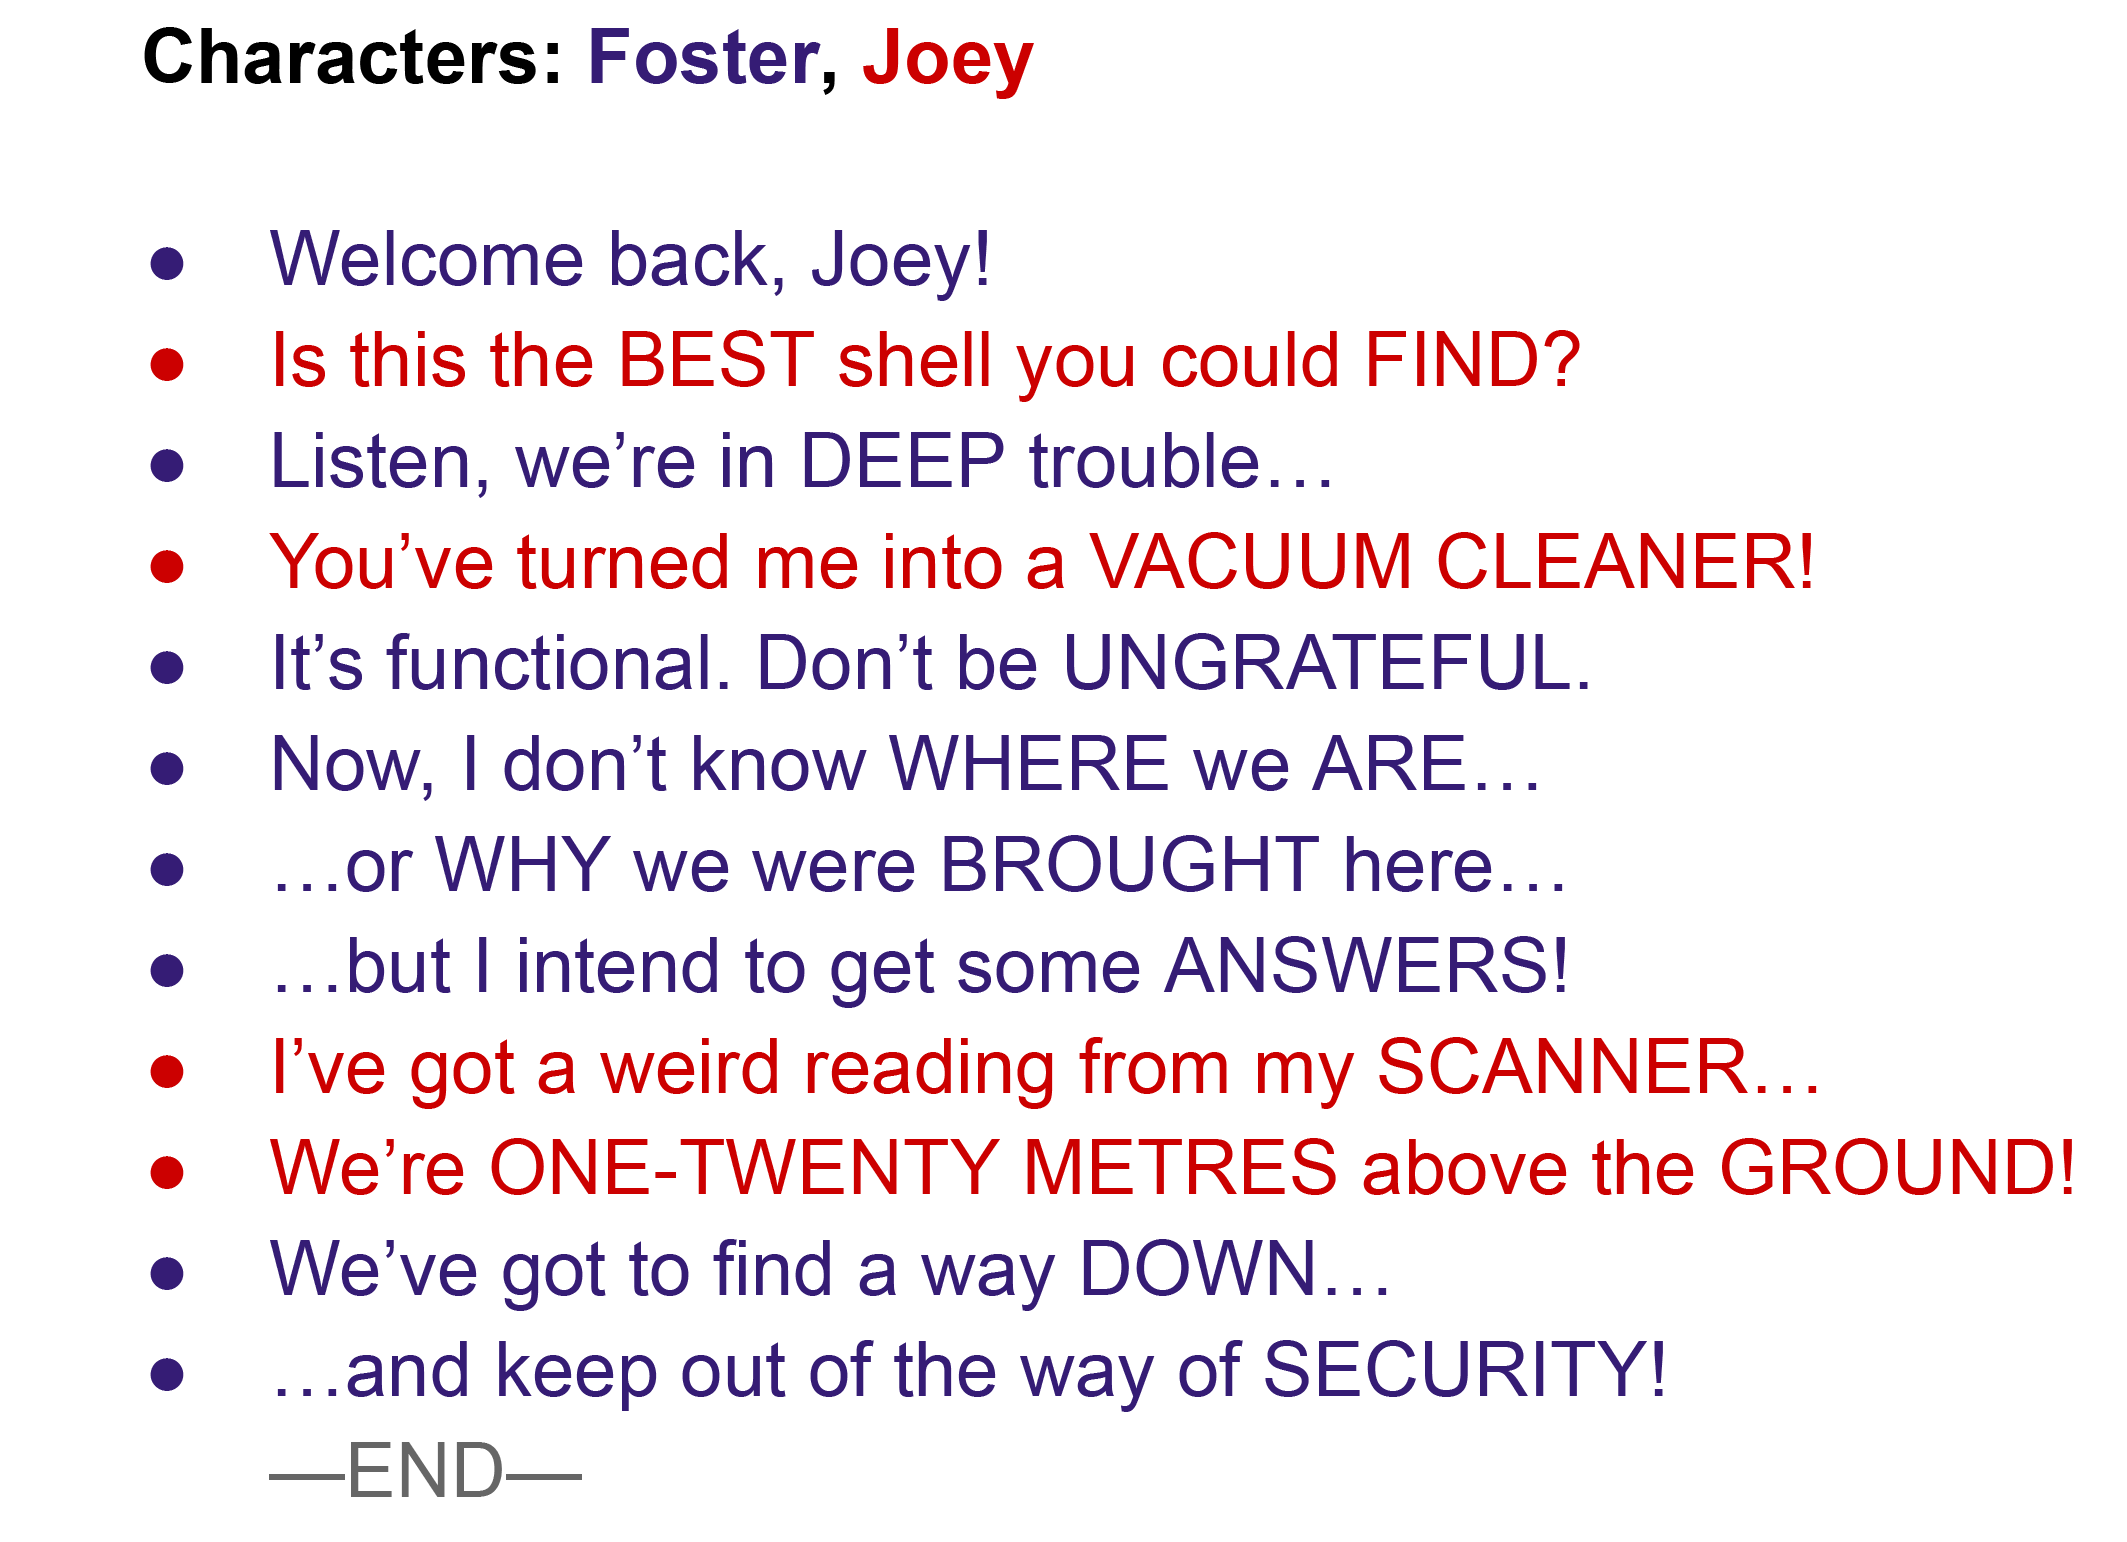
\includegraphics[width=.6\linewidth]{img/dialogueSimple.png}
\caption{A simple conversation between two characters in \textit{Beneath a Steel Sky}.}
\label{fig:DialogueSimple}
\end{figure}

The representation of this conversation in the framework can be fairly straightforward: the dialogue can be stored as a list of data containing the text and other relevant information. In the \textit{Game Dev Beginner} article \cite{Dialogue-French}, John French presents a possible implementation of this approach. However, this linear method has its drawbacks. The complexity increases further when the player is given choices, as shown in Figure \ref{fig:DialogueChoices}. From the start, there are six options A to F the player can select, each branching into a different line of dialogue. When choosing some, like option B for example, the conversation ends the exchange and the option is removed from the list of the six options.  Others, like A, evolve, replacing the original line A1 with a follow-up A2 “\texttt{What IS this place?}”, followed by the return to the list of now updated options. Even though the example depicts a relatively simple interaction, it already highlights the limitations of entering dialogue lines linearly. Adding just a few more branches can result in a tangled structure that becomes nearly unmanageable. The challenge escalates further with the introduction of cyclic paths, where characters may repeat lines based on specific conditions. Representing such behavior using a purely linear format is not only impractical, but also leads to a cluttered and confusing system.

\begin{figure}[H]
\centering
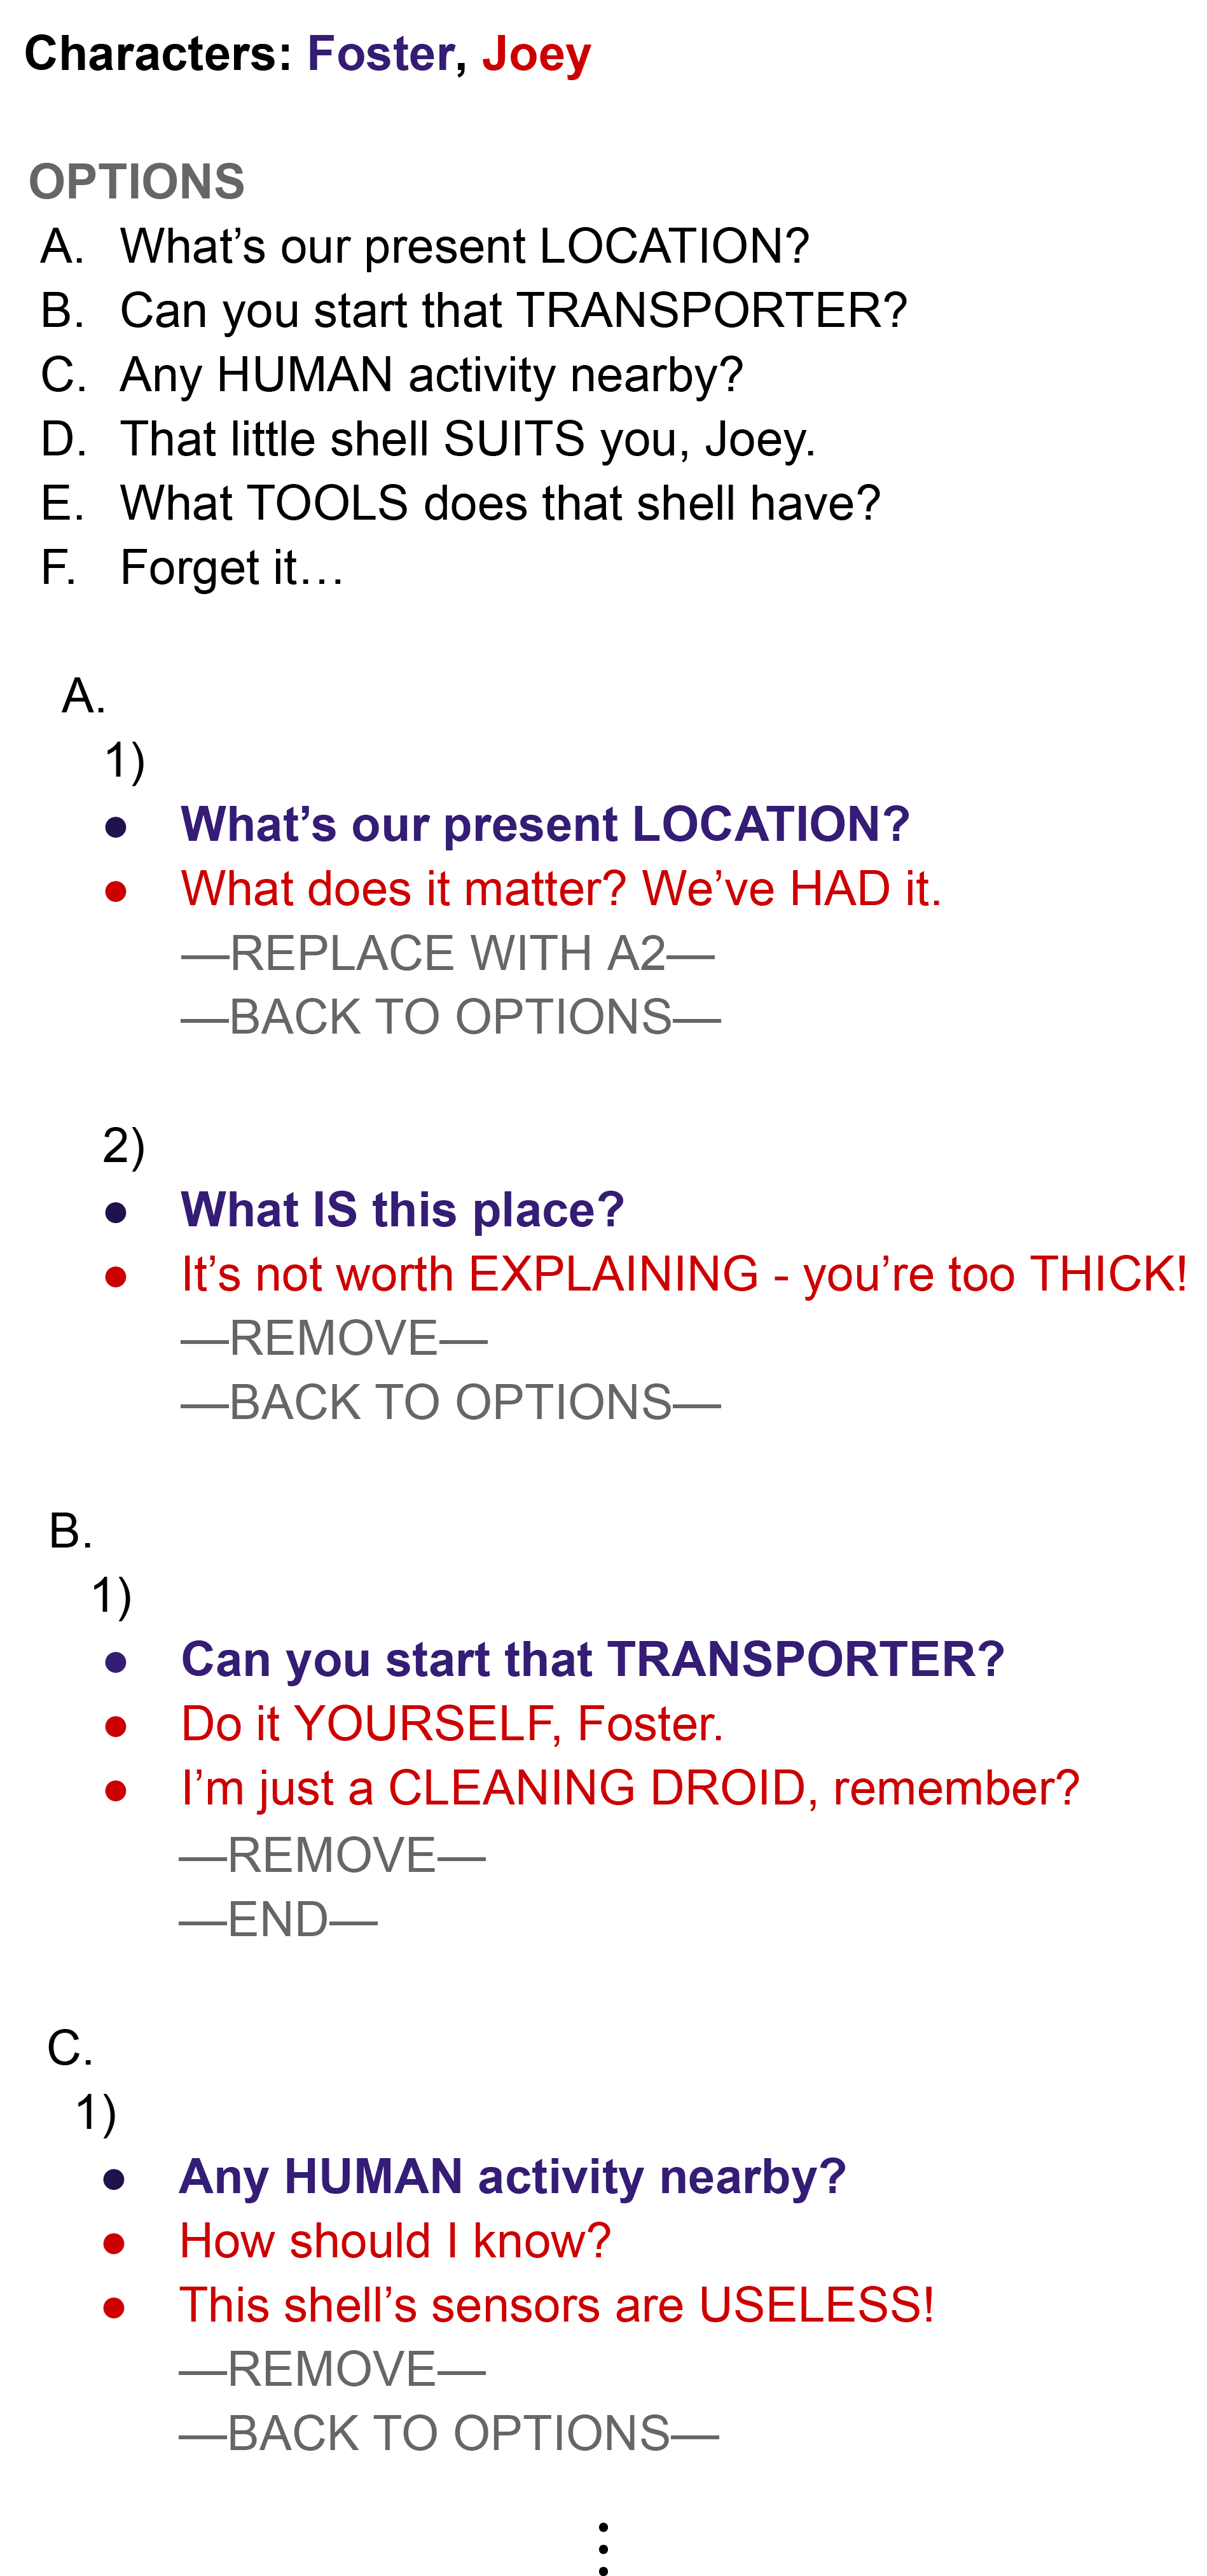
\includegraphics[width=.5\linewidth]{img/DialogueBig3.png}
\caption{A part of a conversation between two characters in \textit{Beneath a Steel Sky}.}
\label{fig:DialogueChoices}
\end{figure}

Due to the limitations of the linear method, it is necessary to explore more flexible solutions. A particular data structure that can effectively represent the complexity of a branching dialogue is a graph. Its structure enables direct access to specific dialogue lines and, in the case of branching paths, offers an intuitive way to manage and visualize the flow. Additionally, graphs make it easy to implement cyclic paths, which can lead to characters reusing parts of the dialogue. All of these advantages are clearly illustrated in Figure \ref{fig:DialogueGraph}, which shows a conversation with multiple branching options represented as a graph. One of the branches even connects to another node across the graph, demonstrating how this structure naturally supports complex and non-linear conversations.

\begin{figure}[H]
\centering
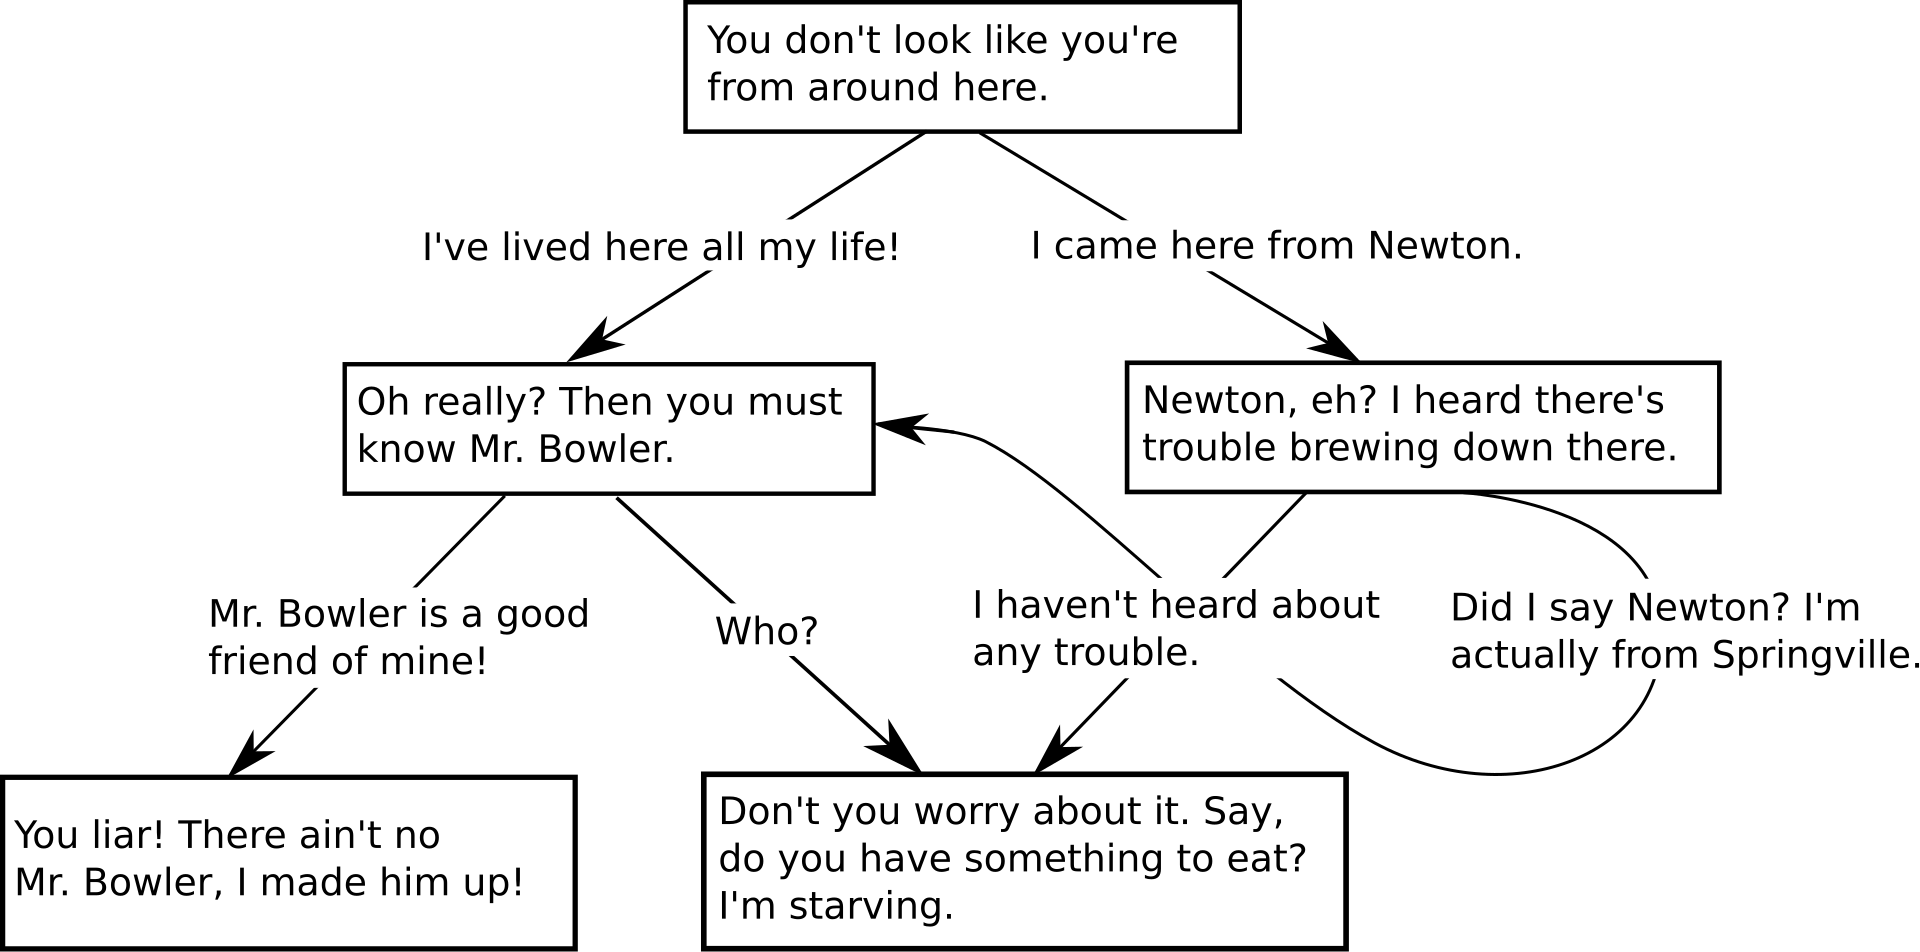
\includegraphics[width=.8\linewidth]{img/image_2025-06-02_133436738.png}
\caption{A conversation with a lot of branching options represented in a graph. Soure: \cite{wiki:DialogueGraph}.}
\label{fig:DialogueGraph}
\end{figure}

Our goal is to design a system that allows for the creation of dialogues in our framework. By using graphs, we can provide users of the framework with a way to manage and edit even complex dialogues in an intuitive and efficient manner. The next step is to determine how such a graph can be represented in Unity. To do this, we will examine the tools Unity provides for working with graphs. 

\subsection{Graph Tools in Unity}
Currently, there is no officially supported non-experimental graph tool or framework available in Unity. A new system named \textit{Graph Toolkit}  \cite{Unity-GraphToolkit} is under development and aims to provide a unified solution for graph-based editing. However, it has not yet been released. Due to the lack of official support, alternative options must be explored. Since one of the core goals of this thesis is to remain free and open source, the tools used should ideally follow the same principles. While the Unity Asset Store offers numerous graph-based tools, many of them do not meet these criteria. Tools such as \textit{FlowCanvas} \cite{FlowCanvas}, \textit{Xtebs Graph Framework} \cite{XtebsGraphFramework}, and \textit{uNode 3 Pro} \cite{uNode3Pro} are all commercial products. On the other hand, \textit{FlowReactor} \cite{FlowReactor} and \textit{xNode} \cite{xNode} are free but have not received updates in several years. \textit{NodeGraphProcessor} \cite{NodeGraphProcessor} emerged as a potential candidate, but its complexity and extensive set of features go beyond the needs of this thesis.

Among the tools offered directly by Unity, we considered \textit{GraphView} \cite{Unity-GraphView} as a possible solution. It is a C\# API provided through Unity’s UI Toolkit framework, designed for building custom, node-based editor tools in Unity Editor. GraphView is commonly used in the creation of visual scripting environments, dialogue systems, shader editors, behavior trees, and similar graph-based tools. However, it remains experimental and lacks official documentation, as it is in the \verb|UnityEditor.Experimental.GraphView| namespace. Notably, NodeGraphProcessor itself is built on top of GraphView, which highlights its utility despite its drawbacks.

Although the current state of graph tool support in Unity is somewhat fragmented, in the end we decided to build a custom graph system using GraphView. Despite its limitations, GraphView continues to enjoy community interest, with recent tutorials drawing significant attention \cite{NodeEditor-YT}. Moreover, it is supported in Unity 6, which makes it usable for at least the near future, up to the release and widespread adoption of the upcoming Graph Toolkit.

For the implementation of the dialogue system, we plan to follow the approach developed by \textit{Kasper Dev Unity}, who created a project \cite{Kasper-Dialogue-Tutorial-git} and a series of tutorials \cite{Kasper-Dialogue-Tutorial-YT} focused on building a dialogue system using Unity’s GraphView API. His method offers a clear and practical foundation for creating node-based dialogue editors, which fits well with the goals of this thesis. While his work will serve as the main reference, we also want to explore other tutorials, such as those by \textit{Mert Kirimgeri} \cite{merpheus-Dialogue-Tutorial-git}\cite{merpheus-Dialogue-Tutorial-YT} and \textit{Indie Wafflus} \cite{Wafflus-Dialogue-Tutorial-git}\cite{Wafflus-Dialogue-Tutorial-YT} to gather different ideas and perspectives. By combining the strengths of these approaches, we aim to build a system that is well suited to the needs of this thesis: flexible enough to handle branching and cyclic dialogue but still simple and intuitive for developers to use. 

\subsection{Features}
\label{Analysis:Dialogue:Features}
Kasper Dev's solution is somewhat more comprehensive than necessary for our purposes, particularly its use of character icons. In Section \ref{sec:Common features}, we closely examined common features of the point-and-click genre and have not encountered such icons. Since they are not essential to our framework, they can be omitted. The same applies to the support for audio clips. As established in Section \ref{sec:Sound_Management}, this thesis does not include the implementation of a sound system, and therefore, the audio functionality can be ignored.

On the other hand, what makes this solution beneficial to our framework is its use of various types of nodes, including the \textit{Start Node}, \textit{End Node}, \textit{Dialogue Node}, \textit{Choice Node}, \textit{Branch Node} and \textit{Event Node}. While their functions are somewhat self-explanatory, a brief overview is still useful:

\begin{itemize}
    \item \textbf{Start Node}
    
This node's only purpose is to mark the starting point of the conversation. It has no predecessor.

    \item \textbf{End Node}

The node indicates the end of a conversation, with options to return to the previous node or restart the last dialogue node. No other node can follow it, meaning that it has no successor.

    \item \textbf{Dialogue Node}

It displays the actual dialogue content. It contains the option to select between the continue types, meaning what the player is supposed to do to progress to the other dialogue nodes: either waiting for a set time or by clicking a continue button. The node also contains the lines of the conversation and can branch to other choice nodes, explained in the following node. It is generally the most frequently used node.

    \item \textbf{Choice Node}

This node presents the player with dialogue choices. Conditions can be assigned to each node whose role is to determine if the choice can be shown or hidden.

    \item \textbf{Branch Node}

It determines which of the two nodes comes next based on specific conditions.

    \item \textbf{Event Node}

The node triggers an in-game event.
\end{itemize}

However, there are certain features missing in Kasper Dev's implementation that would significantly enhance the usability and flexibility of our framework. First, because the dialogue system is closely tied to the player’s actions, such as picking up items or selecting particular dialogue paths, it is important to have a clear and manageable way of tracking those actions. In particular, being able to check whether the player has already selected a specific dialogue option is essential. As illustrated in Figure \ref{fig:DialogueChoices}, selecting one dialogue option can reveal another, making this feature a necessary part of the system. To address this, we take inspiration from \textit{Charles Engine FMV} \cite{CharlesEngine}, a toolkit designed for the development of live-action games. Since this genre puts a heavy emphasis on dialogue, it requires a robust dialogue system, which the \textit{Charles Engine} provides. It solves the issue of dialogue tracking by assigning a \textit{Visited} boolean ScriptableObject| to dialogue nodes \cite{CharlesEngine-tut}. When the player passes through a node, its \textit{Visited} status is set to true, allowing future interactions to reference this information easily.

Another limitation in Kasper Dev's solution is the lack of support for multiple simultaneous text boxes. There are situations in which multiple characters speak at once, such as the example shown in Figure \ref{fig:DialogueConvo}, taken from The Secret of Monkey Island. To accommodate this, we decided to implement a system that allows the addition of an arbitrary number of text boxes, each associated with a corresponding character ID. This approach allows the developer to decide whether multiple characters should speak simultaneously or whether a character should say anything at all, for instance, to create dramatic pauses.

\begin{figure}[H]
\centering
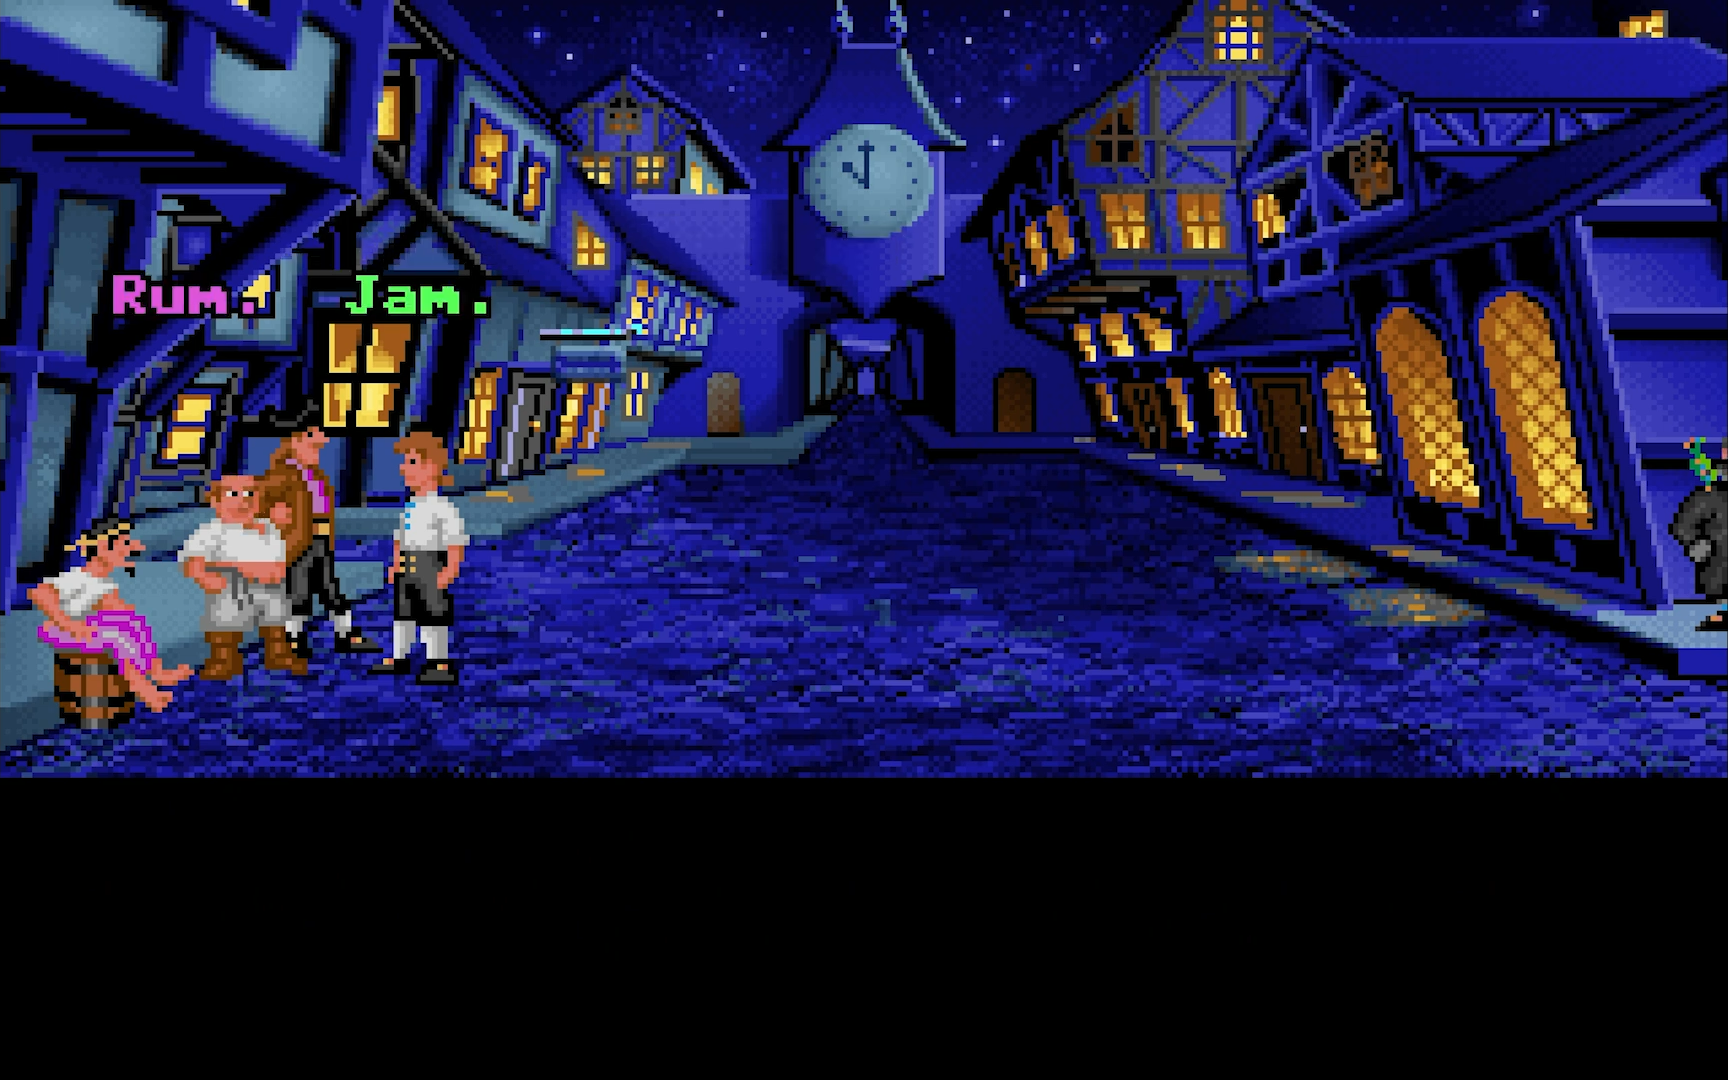
\includegraphics[width=.8\linewidth]{img/Dialogue-talking_at_the_same_time.png}
\caption{The Secret of Monkey Island: A conversation with two characters saying something at the same time.}
\label{fig:DialogueConvo}
\end{figure}

When looking at the other two projects by Mert Kirimgeri and Indie Wafflus, we noticed several small features that would be beneficial for organizing a dialogue graph. Notably, both tutorials introduce the concept of a \textit{minimap}, which is a small floating window that displays a zoomed-out view of the currently edited graph. This gives the developer a better overview of the dialogue flow, especially in large or branching conversations that can easily occur in a 2D point-and-click game. This is why we will include this feature into our framework. 

Additionally, Indie Wafflus implements a feature called \textit{groups}, which allow developers to organize subsets of nodes in the graph. Each group can be assigned a custom name, and dragging the group box moves all nodes it contains, which makes it easier to manage complex dialogue structures. This system is particularly useful when working on nodes which all share a common topic or characteristic, making them thematically or logically connected dialogue blocks. Since dialogue graphs can quickly become complex, this feature offers a valuable and much-needed organization, and so we will implement this feature into the framework as well. 